\documentclass[12pt, twoside, a4paper]{book} % 全局字号12磅
\usepackage[utf8]{inputenc} % 编码格式
\usepackage{graphicx} % 插入图片的,具体不太清楚
\usepackage{times} % times 字体
\usepackage{chapterbib} % 分章节导出参考文献,最终尝试成功,需要在命令行下执行,详见OneNote
\usepackage{dcolumn} % 数学模式制表的包
\usepackage{diagbox} % 制作斜线表头
\usepackage{booktabs} % 三线表制作,命令复杂,不会玩
\usepackage{multirow} % 表格多行控制包
\usepackage{makecell} % 表线控制,较为简单
\usepackage{rotating} % 表格横置的依赖包
\usepackage{colortbl} % 表格上色依赖包
\usepackage{xcolor} % 支持彩色字体
\usepackage{geometry} % 设置纸张大小
\usepackage{amsmath} % 一个公式环境的包,在 begin{matrix} 中可以使用 & 符号进行公式对齐
\usepackage{setspace} % 设置行间距的包,语法:\begin{spacing}{1.25} content \end{spacing}
\usepackage{fancyhdr} % 页眉页脚设置包, 使用简单,但我没用

% 断字和参考文献格式相关
% 使用apa格式参考文献时,使用以下命令。数字格式直接用默认格式, 下边这些需要注释掉,否则报错。
\usepackage[activate={true,nocompatibility}]{microtype} % 不完美解决断行断字问题。参数是自适应调整字间距。keyword: letterspace, hyphenate, expansion, protrusion
\usepackage{cite} % 神奇的包,完美解决引用溢出边界问题。key word: citation, line-breaking
\usepackage{apacite} % APA格式参考文献, 引用格式apacite。目前的问题好像是编译需要多次才能通过。

% 几个没试成功的包
% \usepackage{ragged2e} % 设置两端对齐的,没试成功
% \usepackage{apacite} % 参考文献样式
% \usepackage{newtxtext,newtxmath} % 不知道具体功能,先放进来
% \usepackage[sectionbib]{natbib} % 另一个分章节导出参考文献的包,也没有尝试成功。不过失败原因应该同chapterbib包,已经记录。有时间尝试一下用这个包修改参考文献格式

% 一些全局环境设置
% \setlength{\textwidth} {160 mm} % 设定文本宽度,防止参考文献溢出,无效
\pagestyle{myheadings} % 自定义页眉,显示章节,页码。对于页脚无效
\graphicspath{ {images/} } % 设定图片目录
\renewcommand{\baselinestretch}{1.5} % 基础行间距1.5倍
\setlength{\parskip}{0.7\baselineskip} % 设置段间距
\topskip 10mm % 正文顶部到页眉的距离
% \footskip 5mm % 正文底部到页脚的距离

% 这里设定纸张大小
% PDF VIEW
% \geometry{total={210mm,297mm},
% left=25mm,right=25mm,%
% bindingoffset=0mm, top=25mm,bottom=25mm}

% PRINT
\geometry{total={210mm,297mm},
	left=20mm,right=20mm,
	bindingoffset=10mm, top=25mm,bottom=25mm}

% 调整标题字号行距等
\usepackage{sectsty}
\sectionfont{\fontsize{16}{0}\selectfont}
\subsectionfont{\fontsize{14}{0}\selectfont}
\subsubsectionfont{\fontsize{13}{0}\selectfont}

% 全局调整列表的间距
\usepackage{enumitem}
\setenumerate[1]{itemsep=0pt,partopsep=0pt,parsep=\parskip,topsep=0pt}
\setitemize[1]{itemsep=0pt,partopsep=0pt,parsep=\parskip,topsep=0pt}
\setdescription{itemsep=0pt,partopsep=0pt,parsep=\parskip,topsep=0pt}

% 全文开始
\begin{document}
% 表页制作
\title{
	{\Huge Research on Factors Influencing the Use of Rail Transit}\\
	{\vspace{3cm}}
	{
\includegraphics[width=0.2\linewidth]{university.jpg}}\\
	{\vspace{2cm}}
	{\large Graduate School of Human-Environment Studies}\\
	{\large Kyushu University}
	%{\vspace{1cm}}
}
\author{
	{\large Author: Chen Qi}\\
	{\large Supervisor: Prof. Zhao Shichen}
	{\vspace{1cm}}
}
\date{\normalsize Last Edited: \today}
\maketitle

% 声明页
\centerline{\textbf{\Large STATEMENT}}
%
This academic dissertation is independent research work conducted under the guidance of the supervisor. Except for the quoted content, this dissertation does not contain any research result that has been published by other individuals or groups.\\
\newline
\newline
%
Postscript:
%
This dissertation is edited in \LaTeX. For any details on content or typesetting, please contact below.

\begin{flushright}
	Name: Chen Qi \\
	E-mail: chenqi.clever@gmail.com \\
	QQ: 331730634 \\
\end{flushright}

% 这里设置目录的字体
% \global\large % 设置全局字体,large在12pt文稿下为14.4pt
\renewcommand{\baselinestretch}{1.2} % 目录页基础行间距1.2倍
\fontsize{14pt}{14pt} % 目录字号14pt,行间距局14pt,即1倍基础行距
\selectfont

% 生成目录
\tableofcontents % 内容目录
\listoffigures % 图目录
\listoftables % 表目录

% 这里开始前书部分
\frontmatter

% 设置正文字号
\renewcommand{\baselinestretch}{1.6} % 正文页基础行间距1.8倍
\fontsize{13pt}{13pt} % 正文字号13pt,行间距13pt,即1倍基础行距
\selectfont

% 声明
\chapter{Acknowledgments}
% Most valuable thing duing Ph.D., the overview.
The journey of PhD has both pleasure and pain, but I deeply trust that all I went through today, either good or bad, will be the valuable life experience in the future. If mentioning the most memorable thing during my PhD, maybe I would say the process of shifting the way of thinking from a common people to a researcher, even I can say this is the most valuable thing that I obtained after the 4 years rather than the degree certificate.

% 我要谢!谢全家十八辈儿!
I am not willing to describe the period of PhD in a suffering way, but frankly, I have to say that without the support and help from various people around me, I should have already stopped my feet underway. There are so many thanks I would like to say, please let me express my appreciation one by one.

% 我要谢!一个一个谢!
First and foremost, I would like to thank Prof. Zhao Shichen, my supervisor, for the guidance and instruction not only in my studies but more in work and life attitude. The time of drinking with Prof. Zhao is so joyful and memorable, this drinking time also shortened the distance between us students and professor, for which I appreciated a lot. It's my luck that I came to Zhao laboratory doing research, thank to Prof. Zhao again for teaching me so many things.

% 谢陈思婷帮我搞论文
I would like to thank the fellow students in our laboratory for their feedback on my papers. Communication is an important segment of research, a good research without readers has no meaning. Thanks to everyone for the their patients. Among them, I would like to thank Chen Siting especially for helping a lot in checking English and organizing logic of my papers. 

% 谢日本小鬼子教我日语
Also, I have to say thanks to the cute Japanese fellows, although not for helping me in research. They talked with me, taught me language and culture, made me adapt Japanese life soon. My period in Japan is so enrich and interesting, a large part of which can be attributed to them. In particular, I would like to say thanks to Ikutake Shin, Yoshioka Daiki, Higuchi Go, thanks for their accompany in countless overnights.

% 感谢韩博士家的麻将,火锅,炒菜
One more thing, as we know relax is also important especially during the relatively arduous PhD period, how to spend the boring time and retrieve research condition is always a serious problem puzzling PhD students. Dr. Han Guofeng, my ex-roommate at Kyushu University International House, and his current-roommate provided us the party place in his apartment, where we have hotpot party and even playing mahjong in leisure time. Thanks to my mahjong partners, together with them a lot of happiness is created, boring time is spent, thus accomplishing research with a better status.

% 最后的最重要,我要感谢China, CSC,他们给我钱
The most important thing always come last, all the expense during the 4 years PhD period is sponsored by China Scholarship Council (CSC). With this money, I clearly know that my country is standing behind me, she gives me confidences to step into a new environment, to face the world. Thanks to my country.

% 摘要
\chapter{Abstract}
% 背景
% 城市化带来了一系列的人口,资源,环境的问题,这些问题都可以归结为可持续发展的问题,针对这些问题,TOD被提出,以期能够缓解矛盾
% 说明TOD中,客流预测,以及分析对客流的影响因素是非常必要的。
Urbanization caused many social problems in both developing and developed countries, of which although the problems are different in various ways, in essence, they can be attributed to the demand for sustainability. With the goal of making cities more sustainable, the concept of TOD aiming at compact development was proposed to alleviate the conflict between sustainability and development. However, the implementation of TOD is not as simple as building rail transit stations, then waiting for people to come. Understanding the factors influencing rail transit ridership is always central and fundamental to decisions on urban planning and management at any stage of implementing TOD.

% 主旨,目的
% 因此,本文最基本的目的是解释客流量。具体来看,目的可以分为三个。
This research sets the primary purpose of explaining rail transit ridership in TOD area, from which is expanded to three specific aspects: 1. explaining transit ridership at station level; 2. explaining transit ridership at station-to-station level; 3. explaining the walking duration of to transit stations. To this end, the research questions are as follow: 1. to find an approach for screening effective influencing factors; 2. to describe the relationship of transit ridership between stations and stations; 3. to explore the relation between walking distance and walking preference.

% 具体研究的内容,包含方法
The first question is answered through the exploratory regression decreasing the risk of type I and type II errors in statistic when identifying the valid variables that should be put into the regression model. The specific influence of screened valid variables are then estimated using mixed geographically weighted regression. The results give the factors actually playing a role on influencing transit ridership, and indicate the influence quantitatively. 

For the second question, the relationship of transit ridership between stations and stations is analyzed from the view of land use within the station catchment area. This relationship then is converted into a binary choice problem, and is estimated using logistic regression model. The results show that for passengers the variations in land use in departure stations can lead to variations in the choice of destination stations.

As to the third question, this research examines the feature distribution of individual characteristics at several thresholds of walking duration, thus trying to explore the willingness of walking duration to transit stations. The model of random forest decision is introduced to explain the relationship from the perspective of probability. The results show a quantitative relationship of surveyed walking durations and passengers' individual characteristics, which is thought can be used in planning catchment areas of rail transit station or estimating the catchment areas of existing stations.

% 讨论和建议
Based on the achievements of this research, several recommendations are given as follow: 1. before estimating transit ridership a general process of screening valid factors is necessary; 2. since the transit ridership of one station is not only affected by the factors within the catchment area of that station but also affected by the other stations in the same transit network, the research perspective should be shifted to station-to-station level and further to the line or network level. 3. accuracy estimation for catchment area needs further exploration. \\ \\ \\

\noindent % 不缩进
\textbf{Keywords:} Urban planning; Rail transit ridership; Catchment area; Land use; Individual characteristic; Walking duration

% 正文
\mainmatter % 该命令以下标记为正文,在目录和页码中有所区别

\chapter{General Introduction}
\markright{CHAPTER 1}
%
\section{Background}
% status quo
With the continued urbanization, people continue to migrate from rural areas to urban areas. As a result of this, 54 percent of people worldwide live in urban areas by 2014, this population shift will keep going and is predicted to reach 66\% by 2050 \cite{UN2014world}. Living in cities is considered much more efficient and convenient than that in rural areas in a variety of ways, as it is easier to provide services when people live closer together. However, cities also change the way that humans interact with each other and the environment, often causing multiple problems. The second UN Conference on Human Settlements in 1996 came to the conclusion that the cities all over the world are facing problems due to urbanization.

 
% Different situations in developing countries and developed conutries
Although the problems commonly exist all over the world, the type and scale of problems differ from different stages of urbanization. As to developing countries who are now experiencing a rapid growth in the urbanization, the problems mainly include such as traffic congestion, disorganization, and air pollution, which usually follow by the rapid migrants from rural areas to urban areas. Essentially, most of the problems are caused by the unbalance of demand and supply in land-use, resource, and infrastructure. How to satisfy this demand is an important issue that the governments in developing countries have to consider and address. Different from the situation in developing countries, population aging and low birthrate has become the serious problems in developed countries. With a rapidly increasing proportion of old people in the population, governments are forced to increase expenditure on social security, adding to that the low birthrate, further intensifies the shrinking of working-age population, thus increasing the fiscal burden of governments. How to reduce the public financial expenditure and improve the efficiency of social operation has become a problem that the governments in developed countries have to face. 

% Summary of status quo
In some ways, the problems of the developing countries and the developed countries are very different, but in essence, either of them is the problem of sustainability. While governments in the developing world must try to increase the supply of services to satisfy the increasing population, those in the developed world must try to cope with economic slowdown due to decentralization and changing working patterns. Under such a realistic background, a sustainable program for urban planning seems to be necessary.

% Introduce TOD
In urban planning, transit-oriented development (TOD) is a type of urban development that mix residential, business and leisure space within walking distance of public transport, which was first to be proposed by Calthorpe, Peter in 1993 \cite{calthorpe1993next}. In so doing, TOD aims to increase public transport ridership and by reducing automobile travel, thus promoting sustainable urban growth. As to the precise definition of TOD, while the details vary in scope and specificity, most TOD definitions share several common elements \cite{boarnet1997story,bernick1997transit,megally2001california,cervero2004transit}:

\begin{itemize}
	\item Mixed-use development
	\item Transit stations as cores
	\item Compactness
	\item Pedestrian-friendly
\end{itemize}

% 
Now the guidelines of TOD summarized above has received a lot of attention by all levels of governments as the means of mitigating most of the common urban problems, including traffic congestion, air pollution, and incessant sprawl \cite{cervero2002transit}. In a common sense, an area based on TOD typically has a central transit stop (such as a train station, or light rail or bus stop) surrounded by a high-density mixed-use area, with lower-density areas spreading out from this center. The densest areas of a TOD are normally located within a radius of 400 meters to 800 meters (5 minutes to 10 minutes walking duration, varying by different kinds of public transit) around the central transit stop, as this is considered to be an appropriate scale for pedestrians, thus solving the last mile problem. 

% Change the objective to rail transit station.
% Interpret the importance of ridership prediction
With the increase in demand for speed, punctuality and environment protection, urban rail transit has gained popularity by governments, especially in metropolises with high compactness and population density. Add to the continuous extension of city scale and growth in travel demand, more and more TODs are implemented taking rail transit station as the core. With this popularity, it is probably easy to enter a misunderstanding that if the transit station is built, people will come, but the implementation of TOD is not that simple. Because of this, understanding the factors influencing rail transit ridership is becoming central and fundamental to decisions on urban planning and management under the guidelines of TOD. 

% 
\section{Research purpose}
% propose station level and station-to-station level
What explains rail transit ridership in TOD? As interpreted before, this question is placed in front of us. The answer seems to be both obvious and complex. Every element existing in the catchment area of stations associate with ridership, population, road network, parking, income, transit network, building density, and so on all surely play a role. But the relative importance of these various factors and the internal relations among them are much more complex, and still not well understood \cite{taylor2003factors}. Besides, as transit station is part of transit network rather than a independent existence, once the transit ridership of one station varied, transit ridership of all the other stations connected to that station must vary as well. The interaction among connected stations in the same transit network is still not clear.

%  catchment area
We mentioned the term of catchment area above, however, what does it mean in transit ridership analysis? As a general definition, a catchment area is the area from which a city, service or institution attracts a population that uses its services. In the issue of transit ridership analysis, it means a station's primary service area, within which that people are willing to use the station, beyond which land use, travel mode choice, population distribution are unlikely to be influenced by this transit station. The catchment area is thought to be largely determined by people's willingness of walking to transit stations, which, however, vary by people's individual characteristics including trip purpose, age, gender and so on \cite{guerra2013half}. Obviously, the transit catchment area is important and fundamental to the ridership analysis, even the most.

% 基于上述存在的现实问题,我们得出了explain rail transit ridership 这个整体目标。以此为中心,本文针对以下三个问题点进行展开
Based on the interpretation of the real issue above, the research goal of the whole dissertation is defined to \emph{\textbf{explain rail transit ridership}}. Three questions are to be answered in this dissertation.

\begin{itemize}
	\item What explains transit ridership at station level?
	\item What explains transit ridership at station-to-station level?
	\item What is the correlation between catchment area and walking preference?
\end{itemize}

\section{Literature review} 
% 首先说明该研究通常包含三个点,然后贴那个大表,从三个点展开
% 分问题点的review
From the research purposes, the literature review is to be extended in terms of method, influencing factor, and catchment area respectively. Table \ref{tab:chp1:Review} gives a brief summary for the literature about transit ridership analysis.

% Table 1
\begin{sidewaystable}[htbp]
	\scriptsize % 该表使用小字体
	\renewcommand{\arraystretch}{0.5} % 重设表间距
	\begin{spacing}{0.5} % 这中间行间距0.5倍
		\centering
		\caption{Summary of some previous studies}
		\label{tab:chp1:Review}
		% 这里的格式控制为限制单元格宽度,自动换行,并居中
		\begin{tabular}{|p{8em}<{\centering}|c|p{5em}<{\centering}|p{5em}<{\centering}|p{5em}<{\centering}|p{5em}<{\centering}|p{5em}<{\centering}|p{5em}<{\centering}|p{5em}<{\centering}|p{5em}<{\centering}|p{5em}<{\centering}|p{5em}<{\centering}|}
			\toprule
			\multicolumn{2}{|c|}{Year} & 2004 & 2004 & 2009  & 2010 & 2011 & 2012 & 2013 & 2013 & 2015  \\
			
			\cmidrule{1-11}
			\multicolumn{2}{|c|}{Author} & Chu & Kuby et al. & Taylor et al. & Sohn and Shim & Gutiérrez et al. & Cardozo et al. & Chakraborty et al. & Zhao et al. & Jun et al.  \\
			
			\cmidrule{1-11}
			\multicolumn{2}{|c|}{Catchment} & $1/4$ mile (400m) walking distance & Half mile (800m) walking distance & N/A & N/A & Distance-decay 800m buffer & 800m walking distance & N/A & 800m radius & 300m, 600m, 900m radius  \\
			
			\cmidrule{1-11}
			\multicolumn{2}{|c|}{Method} & Poisson Regression & WLS & 2SLS & OLS, SEM & OLS & OLS, GWR & OLS, SEM & OLS & OLS, MGWR  \\
			
			\cmidrule{1-11}
			\multicolumn{2}{|c|}{Sample Size} & 2568 & 268 & 265 & 251 & 158 & 190 & 900 & 55 & 442  \\
			
			\cmidrule{1-11}
			\multicolumn{2}{|c|}{Number of Valid Indicator} & 15 & 11 & 8 & 7 & 9 & 4 & 9 & 11 & 11  \\
			
			\cmidrule{1-11}
			\multicolumn{2}{|c|}{Coefficient of determination (Adjusted R2)} & 0.54 & 0.71 & 0.91 & 0.6 & 0.73 & 0.56 & 0.69 & 0.95 & 0.77  \\
			\midrule
			
			% 这里的multirow格式控制,限制宽度自动换行,内容部分加上\centering 可以居中
			\multirow{6}[10]{8em}{\centering{Land use factors}} & Building area & & & & $\bullet$ & $\bullet$ & & $\bullet$ & $\bullet$ & $\bullet$  \\
			\cmidrule{2-11}
			& Hospital & & & & & & & & $\bullet$ &  \\
			\cmidrule{2-11}
			& School/University & & & & $\bullet$ & & & & $\bullet$ &  \\
			\cmidrule{2-11}
			& CBD & & $\bullet$ & & & & & & $\bullet$ &  \\
			\cmidrule{2-11}
			& Land use mix & & & & $\bullet$ & $\bullet$ & $\bullet$ & & & $\bullet$ \\
			\cmidrule{2-11}
			& Other infrastructures & & $\bullet$ & & & & & & $\bullet$ & $\bullet$ \\
			
			\midrule
			\multirow{6}[10]{8em}{\centering{Transit-related factors}} & Accessibility of pedestrian & $\bullet$ & & & & & & $\bullet$ & &  \\
			\cmidrule{2-11}
			& Accessibility of transfer & & $\bullet$ & & $\bullet$ & $\bullet$ & $\bullet$ & $\bullet$ & $\bullet$ & $\bullet$ \\
			\cmidrule{2-11}
			& Road coverage & & & $\bullet$ & $\bullet$ & & & & $\bullet$ &  \\
			\cmidrule{2-11}
			& Parking & & $\bullet$ & & & & & & $\bullet$ &  \\
			\cmidrule{2-11}
			& Service level of public transit & $\bullet$ & $\bullet$ & $\bullet$ & & $\bullet$ & $\bullet$ &       & $\bullet$ & $\bullet$ \\
			\cmidrule{2-11}
			& Locational factor & & $\bullet$ & & $\bullet$ & & & & $\bullet$ &  \\
			\midrule
			
			\multirow{8}[12]{8em}{\centering{Demographic and socioeconomic environment factors}} & Population & & $\bullet$ & $\bullet$ & $\bullet$ & & $\bullet$ & $\bullet$ & $\bullet$ & $\bullet$ \\
			\cmidrule{2-11}
			& Employment & $\bullet$ & $\bullet$ & $\bullet$ & $\bullet$ & $\bullet$ & $\bullet$ & $\bullet$ & $\bullet$ & $\bullet$ \\
			\cmidrule{2-11}
			& Age   & $\bullet$ & & $\bullet$ & & & & & & $\bullet$ \\
			\cmidrule{2-11}
			& Tenant proportion & & $\bullet$ & & & & & & & $\bullet$ \\
			\cmidrule{2-11}
			& Race  & $\bullet$ & $\bullet$ & $\bullet$ & & $\bullet$ & & & &  \\
			\cmidrule{2-11}
			& Income & $\bullet$ & & & & & & $\bullet$ & &  \\
			\cmidrule{2-11}
			& Vehicles holdings & $\bullet$ & & & & & $\bullet$ & $\bullet$ & &  \\
			\cmidrule{2-11}
			& Fare  & & & $\bullet$ & & & & & &  \\
			\bottomrule
		\end{tabular}
	\end{spacing}
\end{sidewaystable}

\subsection{Method}
% 阐述一下客流预测的主要方法,最终在TOD下,我选择了station-level的预测。
% 说明一下大家都在作regression,绝大多数都在做单点的预测。
% chp2 和 chp3 内容

% 定位于交通预测模型
From the view of methodology, exploring and estimating the transit ridership can be treated as part of travel demand forecast \cite{miller1999potential,boyce1994introducing}. There are few fields in urban planning paying more attention to the statistical model for looking into the future than transportation. To date, a host of models have been developed and practiced for the issue of transit ridership, of which the most widely used are the activity-based four-step model and the direct model \cite{mcnally2007four,ewing2010travel}. While either of them works on travel demand forecast, they have different application scenario.

% 吐槽四阶段
Traffic Analysis Zones (TAZs), which is a definition in four-step models, range in size from block groups to census tracts, commonly working at macro scales: corridors, subregions, and stats. The resolution of four-step models tends to be too gross to deal with the issues at neighborhood-scale like TOD \cite{cervero2006alternative}. Even though the four-step model has enjoyed widespread support from decades of use, it was never meant to predict the travel demand at neighborhood-scale taking transit stations as cores, not to mention the estimation of influencing factors on the transit ridership \cite{cervero2006alternative,chu2004ridership,duduta2013direct}. Additionally, in the four-step approach, trip generation stage is usually conducted based on an empirical model using some socioeconomic variables like population, employment, auto ownership, however, in different city cases, the impact of traffic indicators will not be exactly the same \cite{jones1983demand}. It is also unclear whether these selected indicators are significantly related to traffic volume, or whether there is an indeed linear relationship between traffic volume and these selected indicators. 

% 狂吹direct model
Direct models estimates ridership as a function of station environments and transit service features based on observed ridership and statistical data \cite{cervero2006alternative}. With the development of geographic information system (GIS) technology and the richness of digital statistic, direct models have gained popularity in estimating travel demand at neighborhood-scale, most notably for TODs. The advantages of direct models firstly stem from the ease of estimation with data that are readily available to transit agencies. The only critical requirements are GIS, statistics for built-environments around stations, and the corresponding transit ridership \cite{guerra2012half}. The advantages are also reflected in the accuracy of prediction, that much easier and faster than other travel demand models, direct models can also provide strong predictive power \cite{lane2006sketch}. Compared with the disadvantage mentioned in four-step models, since the estimation in direct models is based on the historical statistics, it can justify the importance and validity of indicators that are expected to influence transit ridership \cite{walters2003forecasting}.

\subsection{Influencing factor}
% chp2 基本照搬
% 影响transit ridership的因素分为了3类
Transit ridership is generally thought to be related to land use, transportation environment, or travel preferences \cite{thompson1997achieving}. In 1997, Cervero proposed a three dimension index system (Density, Diversity, and Design) to examine the ridership of transit \cite{cervero1997travel}, which has been generally accepted as a basic principle. In addition, many extensions have also been added to the 3D theory, such as accessibility to the station, connectivity of line, and capacity of station \cite{beimborn2003accessibility,garcia2013walking}. In this study, all the candidate factors expected to influence transit ridership can be classified into three main categories: a. land use factors; b. transit-related factors; c. demographic and socioeconomic environment factors.

% land use factors
Land use includes the buildings or facilities that provide the setting for human activity, and it has been widely proved to have a strong relationship with ridership. Also, land use diversity has a significant effect on ridership since it reflects the balance between traffic demand and supply within the catchment area. Although the definitions of land use diversity are not the same according to different researchers, it is widely accepted that higher diversity tends to result in less transit ridership \cite{cardozo2012application,choi2012analysis,gutierrez2011transit,jun2015land,sohn2010factors,sung2014exploring}.

% transit-related factors
Transit-related factors are important for passengers going to take public transit. Better accessibility is thought to be attractive for passengers living further. The factors for accessibility are commonly described as the number of transfers, network density, number of parking facilities and walking convenience \cite{kuby2004factors,sohn2010factors,taylor2009nature,zhao2014analysis,chu2004ridership}. Also, the type and location of a station can affect accessibility as well. Terminal stations are more attractive for passengers because people can accept to spend more time on getting to a terminal station which is easier to transfer to other line or another mode of transportation \cite{o1996walking}.

% demographic and socioeconomic environment factors
The demographic and socioeconomic environment is an important factor which can reflect the travel preference. Obviously, the resident population and employment-population within the catchment area are crucial factors on ridership of the subway station. Besides, the economic factors also play an important role in ridership. For example, in the area where the car ownership is higher, people are more likely to choose private car than public transit \cite{chiou2015factors,zhao2005transit}; also the higher the percentage of low-income household is, the more likely people tend to take public transit \cite{thompson2012really}. Furthermore, the ratio of apartments and rental house within catchment have been verified being relevant with ridership in some degree \cite{jun2015land}.

\subsection{Catchment area}
% chp2 和 chp4 的整合。首先800米的论述,然后说明其实这个并不是这样
% 这部分写的太烂啦,第一段说明大家都在做什么
% historically,buffer area,PCA
An important precondition for investigating factors influencing transit ridership is the definition of the catchment area of a station, which has been interpreted in the part of research purpose. Historically, the determination of transit catchment area was mainly implemented in GIS by creating a distance buffer around the transit station \cite{o1992analysis,hsiao1997use,ayvalik2002heuristic,peng1997simultaneous}. However, since a transit catchment area is determined by the walking distance from the transit station, which is also called pedestrian catchment area (Abbreviated as PCA), a circle buffer area is not adequate for presenting the catchment area. Recent decades, with the development in GIS and the richness in statistics, the application scenario of GIS has progressed far beyond the simple buffering operation \cite{biba2010new,wu2003ptal,jiang2012walk}. Also, many efforts have been made to estimate the real walking distance by importing the data of real road network. According to the existing studies, the PCA generally range from 400 meters to 1000 meters due to different station types, city forms, also travel preference \cite{alshalalfah2007case,guerra2012half,keijer2000people,murray1998public,o1996walking,zhao2003forecasting}.

% 这里给出支持800米
% 这里给出这个800米其实也很不合理
Since difficulties in estimating the accuracy catchment area are still not well addressed, a general 800 meters (half-mile) walking distance, which has been verified to be suitable for most cases, has been widely accepted as a principal reference of the catchment \cite{kuby2004factors,gutierrez2011transit,cardozo2012application,zhao2013influences}. This 800 meters, however, is just a general distance for rail transit stations without considerations of people's individual characteristics and travel preference. The catchment area is mainly determined on the base of questionnaires by asking how far/long did passengers walk to stations, or how far/long are passengers willing to walk to stations \cite{keijer2000people,zhao2003forecasting,garcia2013walking}, while the answers are usually given in a loose way like I remember I walked... or I think I prefer... What's more, the same reasoning has been used to justify other rail transit catchment areas and even in different cities and countries. Till now, restricted by analytical method and data, there are no better options than this general 800 meters walking distance in determining rail transit catchment area, unless doing a large-scale rail transit travel survey which is also thought to be impossible due to excessive costs.

\subsection{Summary}
To sum up in brief, 
% 该领域的研究尽管已经取得了相当的进展,但在模型,指标,范围这些具体问题上都仍有进一步发展的可能。研究的方向上来看,目前为止的绝大多数研究都还是专注于单个站点问题的挖掘,从线路和网络角度出发的研究非常少。具体来看,direct model在模型上的创新没有什么太大的进展,基本上都是基于regression的改进,并没有从本质上提高。在影响因素的研究上,学者们对于指标的总结归类已经做的非常全面,但对于不同的国家,地区,甚至TOD区域,其影响因素也不尽相同。如何在潜在影响因素中寻找出有效因素这一过程还有待进一步发展。PCA的研究中还有很大的不确定性,无论是视点,方法都有待进一步探索。在对既有文献的充分掌握上,本文将从以下3个研究点展开。

% 2. 探索筛选有效指标的方法。
% 3. 转换研究视点,建立站与站之间关系的模型
% 4. 探寻catchment area 和 walking preference的关系,试图对catchment area进行解释

\section{Dissertation organization}
% 研究范围,案例的简介
% 本文选择了日本福冈作为研究案例,这里附上福冈简介。
% 同时列出数据简介

% 章节划分
\clearpage % 新起一页
\bibliographystyle{apacite}
% 这里需要指定main文件所在路径的相对路径,否则无法读取参考文献。多个bib文件用comma分隔,没有空格
\bibliography{chapters/ref}

\chapter{Chapter 2}


\chapter{Analysis on the characteristics of transit ridership and land use}
\markright{CHAPTER 3}
%
\section{Introduction}
%
\subsection{Background}
%
In recent years, the problem of aging population has occurred in many developed countries, which also always accompanied with decline in population. As a local central city, Fukuoka now is still in the population growth period, the population has reached 1.5 million, nevertheless, the proportion of aging population is continuously increasing as well. According to the census data, it is expected that the population will reach the peak in 15 years and shift to the population decline period, moreover, the aging population will break through one quarter of the total after 10 years (as shown in Figure \ref{fig:chp3:PopulationChange}). On the other hand, the data from Kitakyushu Person Trip Survey shows an inclination of that the private car share rate will keep on increasing while the rail transit share rate will turn to decrease in the future (refer to Figure \ref{fig:chp3:TrafficModeShare}), As a result, this trend of the shift in population structure and traffic share rate will lead to a decline operating income and increase in financial pressure for rail transit operator of Fukuoka, the same problem will also occur in most of the local central cities similar with Fukuoka. Addition to the financial problem for rail transit operators, traffic congestion is also becoming the problem for all the resident. Figure \ref{fig:chp3:TravelSpeed}, which is quoted from Road Traffic Census (2010), shows the average travel speed during crowded time in major cities of Japan. As we can know from this figure, the problem of traffic congestion is becoming more and more serious in the downtown area of Fukuoka.

%
\begin{figure}[htbp]
	\centering
	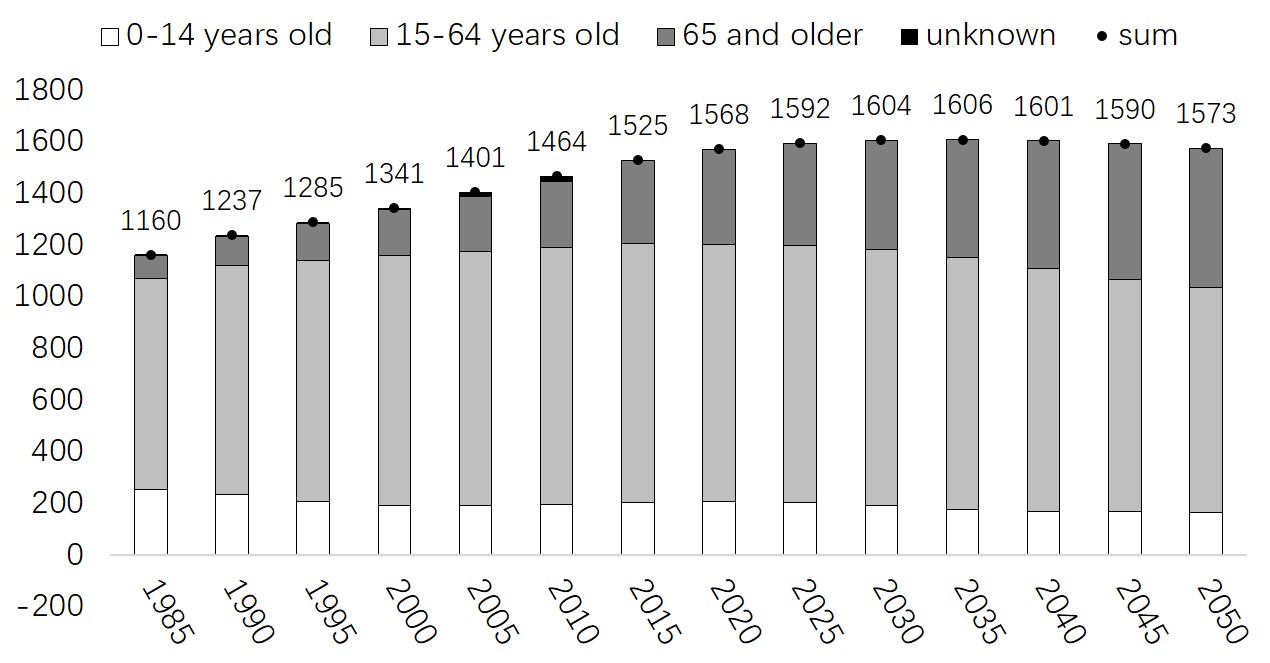
\includegraphics[width=\linewidth]{chapter3/PopulationChange}
	\caption{Trends of population change}
	\label{fig:chp3:PopulationChange}
\end{figure}

%
\begin{figure}[htbp]
	\centering
	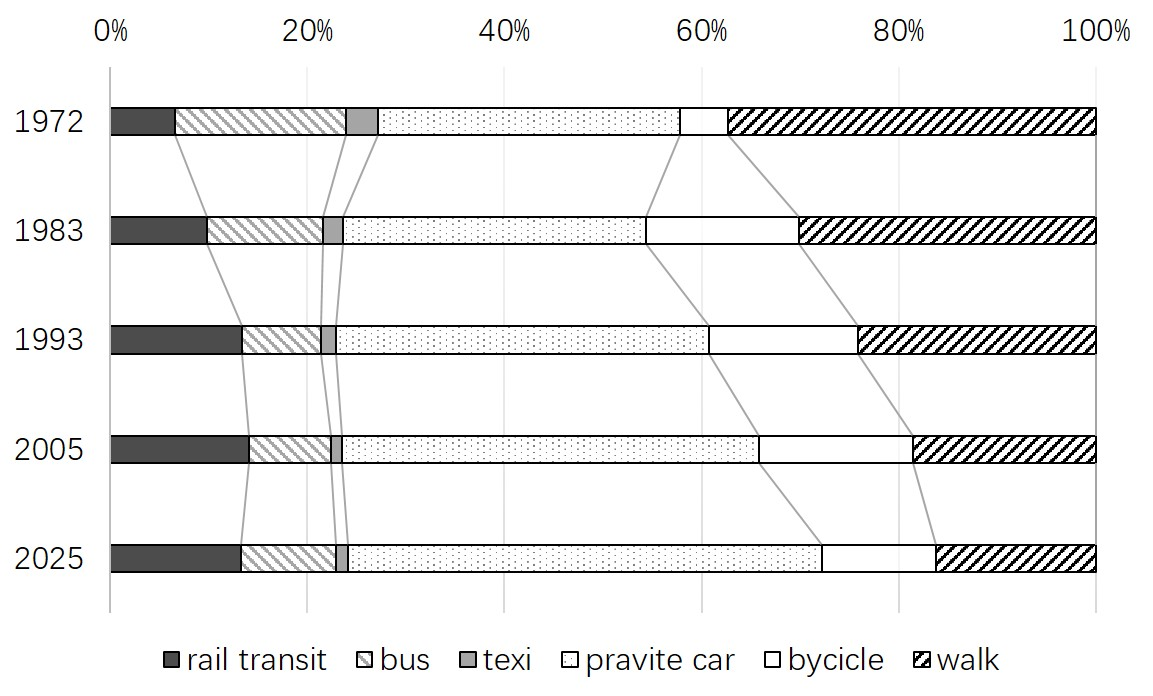
\includegraphics[width=\linewidth]{chapter3/TrafficModeShare}
	\caption{Traffic mode share rate}
	\label{fig:chp3:TrafficModeShare}
\end{figure}

%
\begin{figure}[htbp]
	\centering
	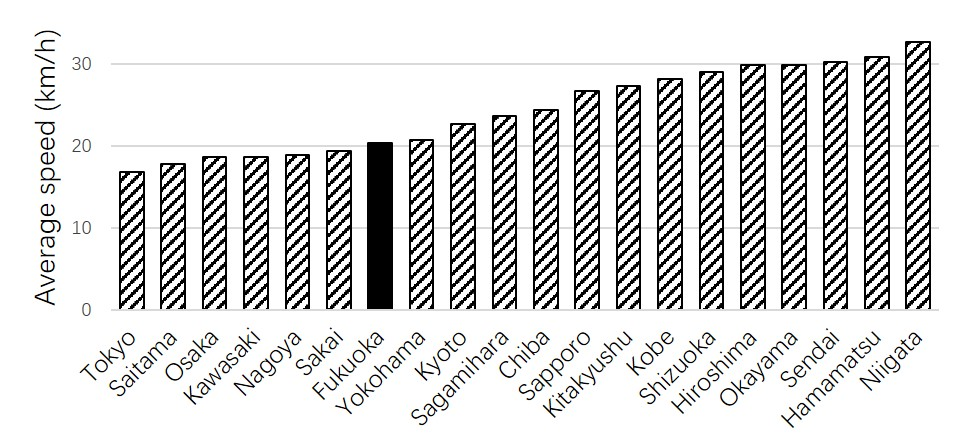
\includegraphics[width=\linewidth]{chapter3/TravelSpeed}
	\caption{Private car travel speed ranking}
	\label{fig:chp3:TravelSpeed}
\end{figure}

%
According to the situation stated above, obviously, the issue put in front of the local central cities like Fukuoka is how to promote the use of rail transit, thus reversing the financial dilemma of rail transit operator and making a better living environment for the resident. To achieve this goal, it is necessary to make clear what factors can influence the rail transit ridership, based on which to make new policy helping improve the role of rail transit.

%
\subsection{Previous studies}
%
Many works have been done on the topic of rail transit ridership and the environment around transit stations, while most of them focused on the trend of variation in rail transit ridership or land use, concentration on the studies of the relationship between the transit ridership and land use is still inadequate \cite{matsumoto2013study,nakamura2015study}. 

%
Depending on the research purpose, the research scale is also different. For example, the study on the changing trends in transit ridership at the scale of Shinkansen mainly aims at making clear the role of each city from the view of entire country \cite{matsumoto2013study}. At a relative small research scale, for example, some studies focused on the urban rail transit within metropolitan area to make clear of the changing trends in urban structure \cite{song2013evaluation,baba2012change}. This study further narrows the research scale to the urban rail transit within cities, mainly focusing on making clear of the changing trends in rail transit ridership itself, thus providing reference for making policies of urban planning and management \cite{nakamura2015study,yano2008}. 

%
Land use around transit stations is always thought as the key factor influencing the transit ridership, while on the other hand, land use is also though to be affected by the transit station. The changes in distribution and types of shop around transit stations are generally considered as good ways to reflect the influence on land use impacted by the stations, the conclusion from existing studies also supported this argument for that the changes of shops around transit stations showed clear characteristics \cite{sui2013research,zhao2012study,kitayama2008study}. The other kinds of facilities belong to different land use is also relate to rail transit ridership, such as clinic, school, and some other public facilities \cite{lee1995predicting,lee1994temporal}. 

%
Some studies also analyzed the influence on transit ridership from the perspective of land use. A study on the changing trend of transit ridership gave the main conclusion that mixed land use around rail transit stations has a constant effect on increasing transit ridership \cite{nakamura2015study}. Quantitative analysis on the relationship between transit ridership and land use usually conducted using regression model (refer to Table \ref{tab:chp1:Review}), which is also applied on the case of Japanese cities. A study using the case of rail transit stations within Tokyo metropolitan showed a result that the land use of residence, office, and education plays the most important role in affecting the transit ridership \cite{tadakatsu2015empirical}.

%
Land use is widely accepted as one of the most important factors influencing transit ridership, nevertheless, the problem is how to find the specific factors of land use to estimate transit ridership, and how to evaluate this effect quantitatively and precisely. Besides, the influencing factors are not only land use, some other factors such as road network, floor area ratio, transfer structure etc. also have an interactive relationship with rail transit ridership \cite{kondo2010railway,inohae2009study}. There are also many factors, even though which has not been fully confirmed yet, maybe also play the important role in determining transit ridership.

%
\subsection{Research purpose}
%
With the goal of promoting the use of rail transit, this chapter focuses on making clear of the characteristics of annual changing in both rail transit ridership and land use around the station, based on which to explore the relationship between transit ridership and land use. 

%
Specifically, the research has two main purposes: 
\begin{enumerate}
	\setlength{\parskip}{0\baselineskip} % 设置段间距
	\item To describe the characteristics of transit stations in terms of both transit ridership and land use.  
	\item To explore the relationship between transit ridership and land use on the base of intensive description on the characteristics of transit stations. 
	\setlength{\parskip}{0.7\baselineskip} % 设置段间距
\end{enumerate}

%
\subsection{Research objects}
%
The research objects in this study is the 35 subway stations of Fukuoka, and several reasons are given here for doing this:

%
\begin{enumerate}
	\setlength{\parskip}{0\baselineskip} % 设置段间距
	\item The catchment area of subway stations cover all the downtown area of Fukuoka, and most of the urban area. 
	\item Subway system undertakes the major rail transit traffic within the urban area of Fukuoka. 
	\item Since subway system is not serving the traffic of intercity, the influencing factors on transit ridership can be easily confined within the area around transit stations, which is conductive to the analysis on the relationship between transit ridership and land use.
	\setlength{\parskip}{0.7\baselineskip} % 设置段间距
\end{enumerate}

%
This study works on the transit ridership and the land use around transit stations, but how to define the area of “around”? Since this study is not aiming at predicting transit ridership using land use factors, the main purpose is to understand the trend of variation in transit ridership and land use and to explore what kind of land use factors can influence the rail transit ridership.



%
\section{Data}
\subsection{Study case introduction}
%
The study case in this study is the subway system of Fukuoka, some details is shown in Table \ref{tab:chp3:SubwayLineInfo}. It consists of three subway lines, the Kukou, or Airport Line (Line 1), the Hakozaki Line (Line 2) and the Nanakuma Line (Line 3). The three lines are operated by the Fukuoka City Transportation Bureau, this subway system is not a large-scale one, which only has 35 stations in total. The distribution and name of the 35 stations is shown in Figure \ref{fig:chp3:SubwayStations}.

% Table
\begin{table}[htbp]
	\centering
	\caption{Information of Fukuoka subway stations}
	\label{tab:chp3:SubwayLineInfo}
	\small
	\renewcommand{\arraystretch}{1.25} % 重设表间距
	\begin{tabular}{ccp{5em}<{\centering}p{4em}<{\centering}p{4em}<{\raggedleft}p{3em}<{\centering}p{4em}<{\centering}}
		\Xhline{1.5pt}
		Line & \multicolumn{1}{c}{Name} & First section opened & Last extended & \multicolumn{1}{c}{Length} & Stations & Gauge \\
		
		\midrule
		1 & Kukou Line & 1981 & 1993 & 13.1 $km$ & 13 & 1067 $mm$\\
		2 & Hakozaki Line & 1982 & 1986 & 4.7 $km$ & 7 & 1067 $mm$ \\
		3 & Nanakuma Line & 2005 & - & 12.0 $km$ & 16 & 1435 $mm$ \\
		\multicolumn{2}{r}{Total} & - & - & 29.8 $km$ & 35 & - \\
		\Xhline{1.5pt}
	\end{tabular}
\end{table}

\begin{figure}[htbp]
	\centering
	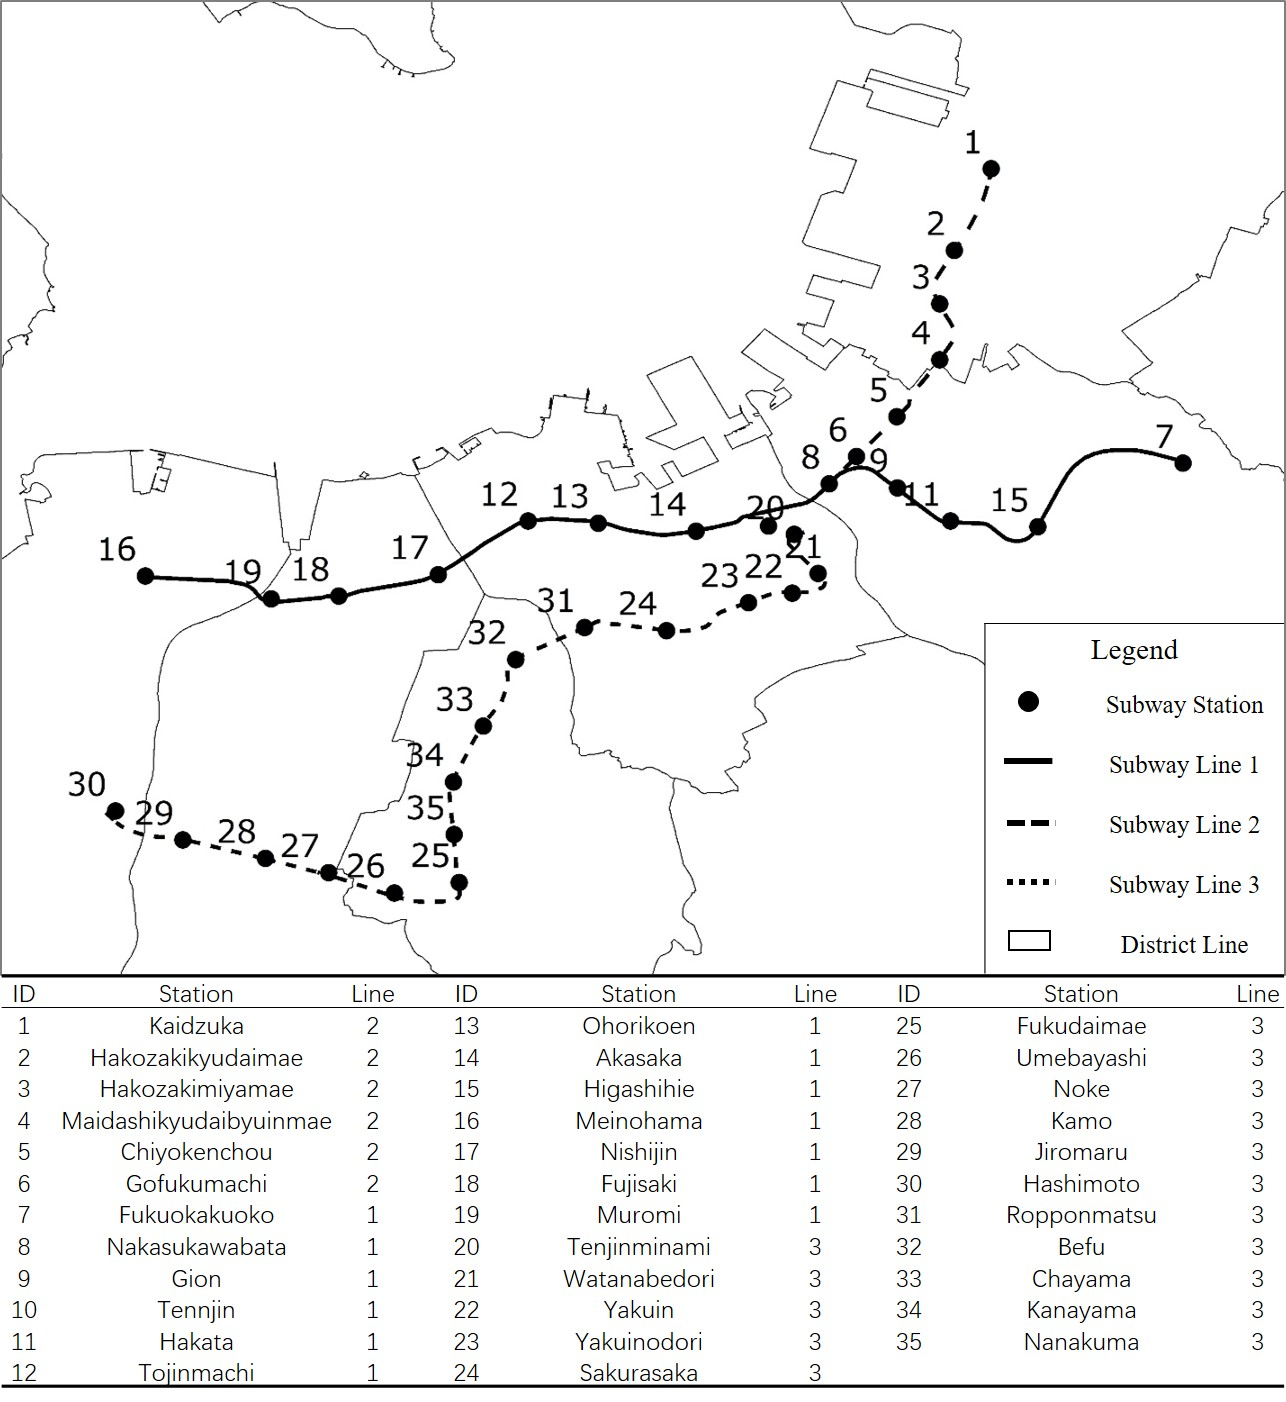
\includegraphics[width=\linewidth]{chapter3/SubwayStations}
	\caption{Distribution of the subway stations}
	\label{fig:chp3:SubwayStations}
\end{figure}

%
From the spatial distribution, the subway stations covered most of the core area of Fukuoka, Line 1 and Line 2 are connected while Line 3 is separated from the other two lines. The catchment area of stations with the number of 8, 9, 10, 11, 20 covers the downtown area, where has the higher density in both population and building. The No. 7 station is in Fukuoka airport, which mainly serves for the transfer of airport passengers. The No. 11 station, Hakata Station, is the comprehensive railway transportation hub of Fukuoka integrating Shinkansen, JR, subway, and bus terminal. The No. 10 station, Tenjin Station, is another central transportation hub, including West Japan Railway, subway, and bus terminal. The two transportation hubs undertake the role as the passenger distribution center not only within Fukuoka urban area but also extending to the cities around Fukuoka city. The endpoint stations with No. 1 and No. 16 connect to other railway lines extending to other cities.

%
\subsection{Data collection}
%
All the dataset used in this study comes from the official statistics, details for the dataset is listed in Table \ref{tab:chp3:DataSource}. The data of subway transit and population is annual statistics, while the data of urban planning basic survey is provided every 5 years. Since the subway line 3 is opened in 2005, the research period is set to the 10 years after the subway line 3 is operated. The statistics of population and land use is on the accuracy of town-chome, which is the smallest region in Japanese administrative division. 

% Table
\begin{table}[htbp]
	\centering
	\caption{Data source}
	\label{tab:chp3:DataSource}%
	\small
	\renewcommand{\arraystretch}{1.25} % 重设表间距
	\begin{tabular}{llll}
		\Xhline{1.5pt}
		Item & Source & Data accuracy & Time point \\
		
		\midrule
		Subway transit ridership & Fukuoka Traffic Bureau & Station & 2005-2014 \\
		Population & Resident Basic Account & Town-chome & 2005-2014 \\
		Land use & Urban Planning Basic Survey & Building & 2003, 2008, 2012 \\
		\Xhline{1.5pt}
	\end{tabular}%

\end{table}%

%
\subsection{Data preprocessing}
%
Since the data accuracy is not matched with population and land use, a preprocess is necessary before conducting the analysis. The data preprocess can be separated into 3 aspects.

%
\begin{enumerate}
	\setlength{\parskip}{0\baselineskip} % 设置段间距
	\item Matching the region of data. Due to the data accuracy of land use is higher than that of population, the common data accuracy is set to town-chome in this study.
	\item Matching the time points of data. To match the time point among different data sources, this study investigates the relationship between transit ridership and land use using the data of 2008, for which is included in all kinds of data.
	\item Extracting the data of population and land use within the catchment area of subway stations. This operation is conducted by using ArcGIS, as shown in Figure \ref{fig:chp3:DataExtraction}, an 800-meter circle area taking the subway station as the center is drawn at first, then the statistics within this area is extracted.
	\setlength{\parskip}{0.7\baselineskip} % 设置段间距
\end{enumerate}

\begin{figure}[htbp]
	\centering
	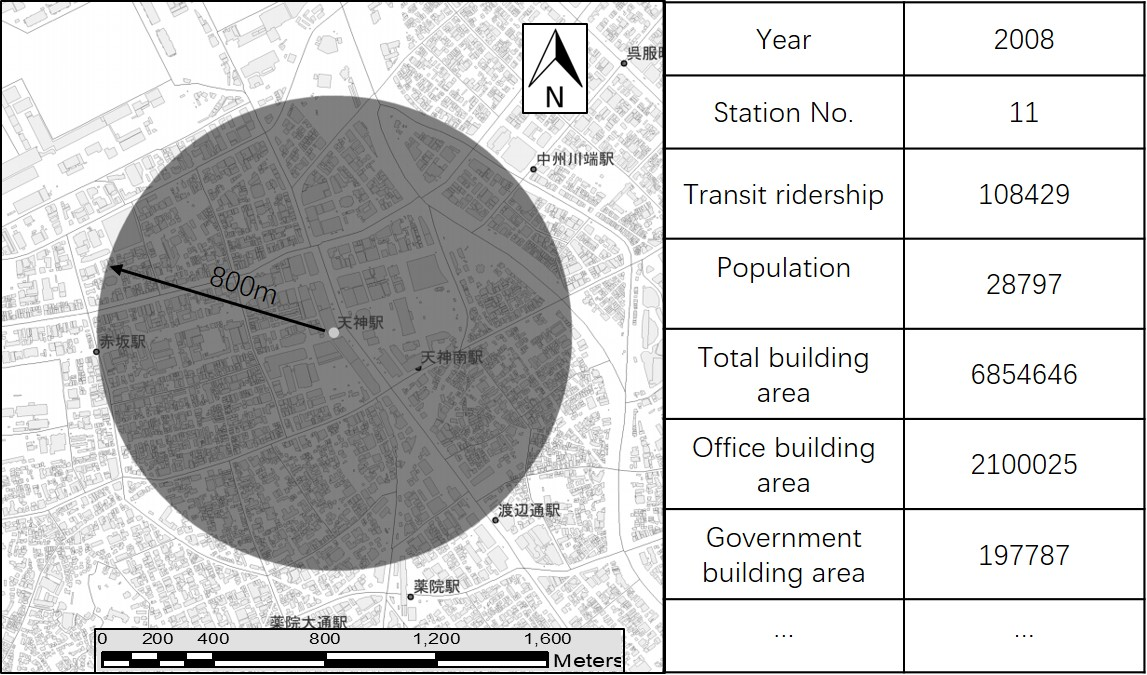
\includegraphics[width=\linewidth]{chapter3/DataExtraction}
	\caption{Extraction of data}
	\label{fig:chp3:DataExtraction}
\end{figure}

%
\section{Characteristics of transit ridership and land use}
%
\subsection{Characteristics of annual change in transit ridership}
%
The subway line 3 was put into operation from 2004, the data of transit ridership was fully recorded from the year of 2005. Figure \ref{fig:chp3:RidershipVariation} gives the trend of transit ridership during 2005-2014. The total transit ridership has exceeded 0.6 million per day, of which the transit ridership of line 1 accounts for the most reaching about 0.5 million per day.

\begin{figure}[htbp]
	\centering
	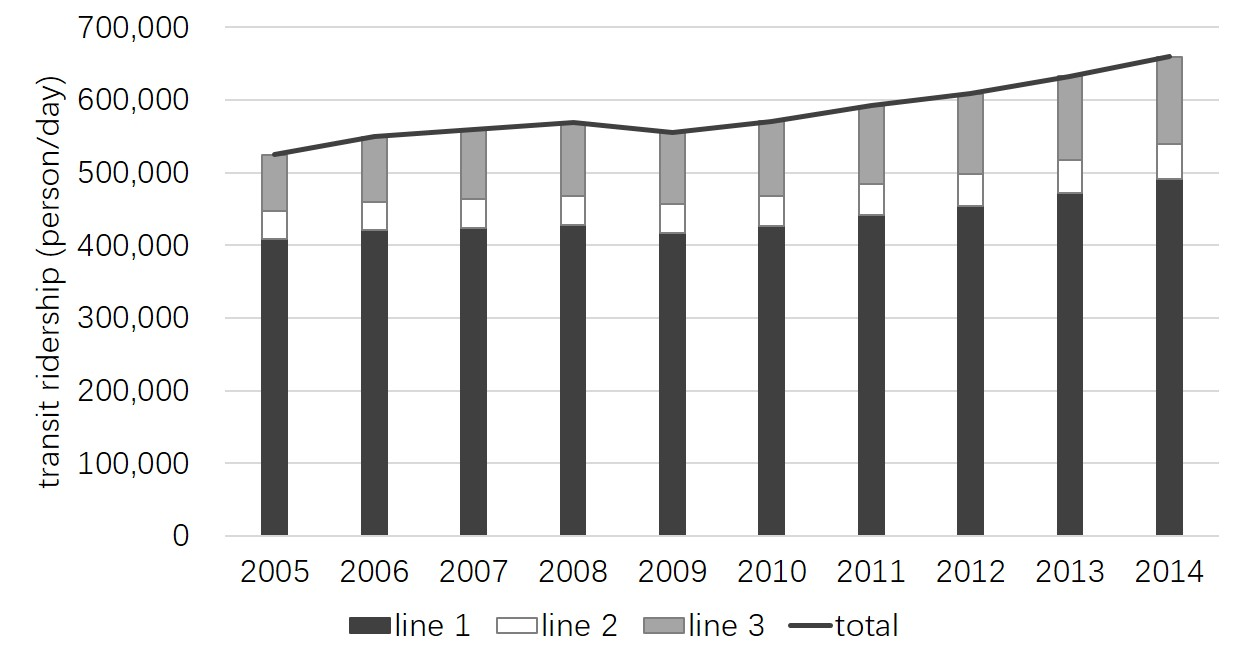
\includegraphics[width=\linewidth]{chapter3/RidershipVariation}
	\caption{Variation in the transit ridership of Fukuoka subway 2005-2014}
	\label{fig:chp3:RidershipVariation}
\end{figure}

%
From the annual change rate of transit ridership in terms of subway lines, as shown in Figure \ref{fig:chp3:AnnualGrowth}, notably, at the first three years after the line 3 was opened, the growth rate of line 3 is much higher than that of line 1 and line 2. After the year of 2009, the growth rates of three lines tend to be stable and consistent with each other.

%
\begin{figure}[htbp]
	\centering
	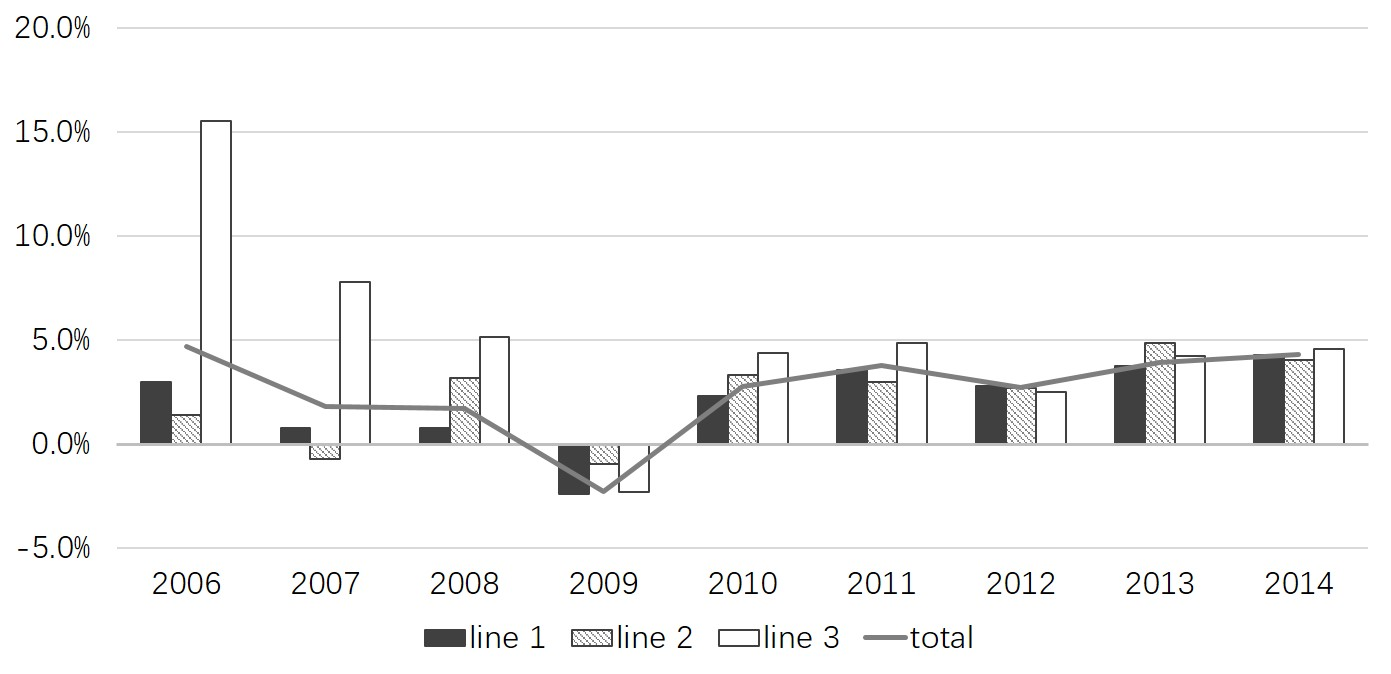
\includegraphics[width=\linewidth]{chapter3/AnnualGrowth}
	\caption{Annual growth rate of transit ridership by subway lines}
	\label{fig:chp3:AnnualGrowth}
\end{figure}

%
The characteristics of transit ridership are investigated from two aspects, the growth rate variation and transit ridership variation. Different types of station have different characteristics, specific to each subway station, the transit ridership and growth rate is as shown in Figure \ref{fig:chp3:AnnualVariationEachStation}, which is sorted by ascending order on transit ridership. The transit ridership is the daily average on the year of 2010, the growth rate is the average of 10 years from 2005 to 2014. 

%
\begin{figure}[htbp]
	\centering
	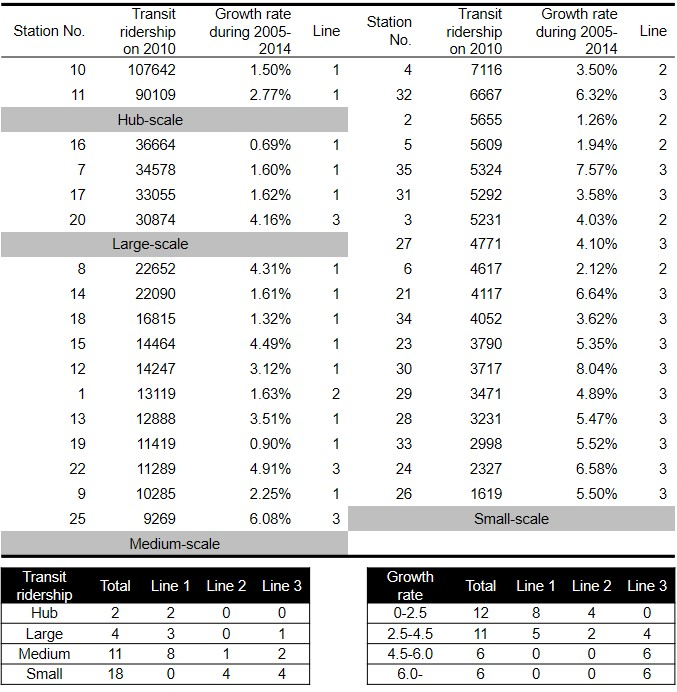
\includegraphics[width=\linewidth]{chapter3/AnnualVariationEachStation}
	\caption{Variation in transit ridership of each station}
	\label{fig:chp3:AnnualVariationEachStation}
\end{figure}

%
Figure \ref{fig:chp3:RidershipSpatialDistribution} plotted the information of each station on the map, the stations in the newly opened line 3 generally have lower transit ridership but higher growth rate. The stations with the higher growth rate in line 1 and line 2 are mainly located close to the downtown area. From the spatial distribution of both transit ridership and growth rate, it shows a clear central agglomeration effect, which means the large-scale stations can attract more passengers.

%
\begin{figure}[htbp]
	\centering
	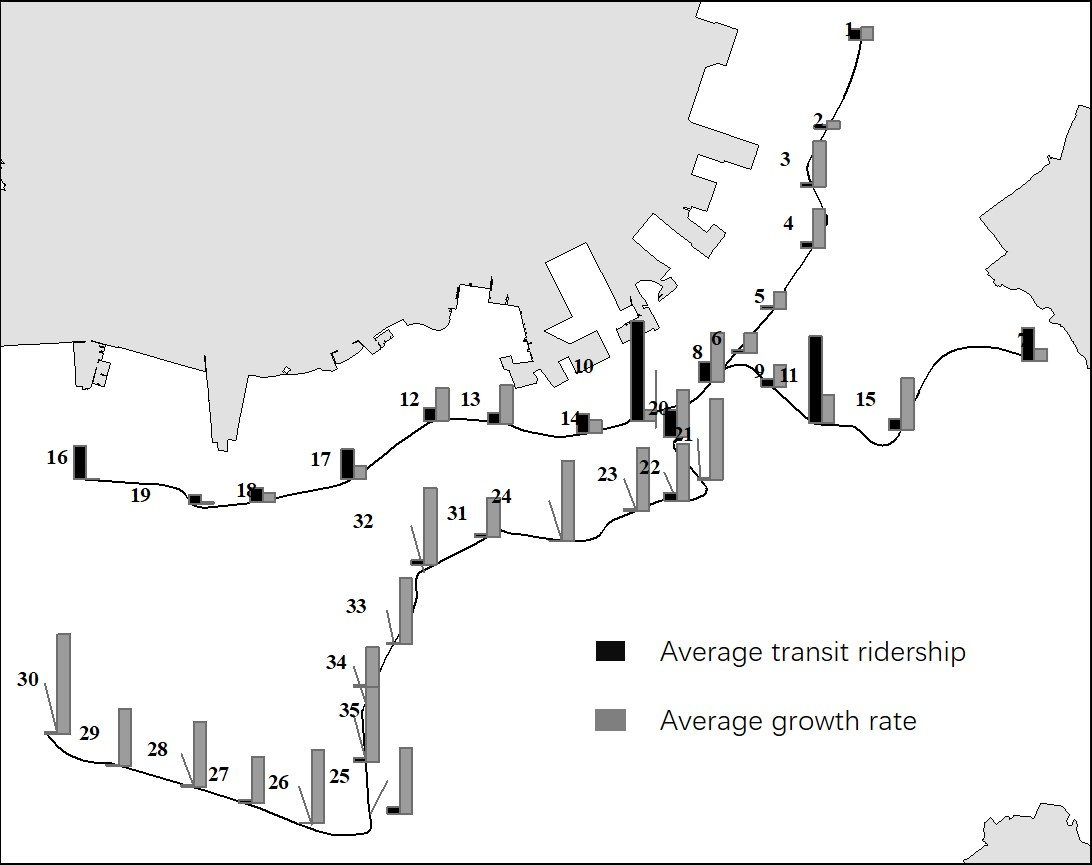
\includegraphics[width=\linewidth]{chapter3/RidershipSpatialDistribution}
	\caption{Spatial distribution of transit ridership}
	\label{fig:chp3:RidershipSpatialDistribution}
\end{figure}

%
\subsection{Analysis on the factors of land use around subway stations}
%
\subsubsection{Data extraction}
%
As stated before, the data of land use is extracted within the 800-meter circle region taking subway station as the center. As shown in the Figure \ref{fig:chp3:BufferAreas}, 35 buffer areas with a 800 meters radius are created. This process of drawing the buffer area and extracting data is conducted using the tool of “Buffer” and “Tabulate Intersection” respectively in ArcGIS.

%
\begin{figure}[htbp]
	\centering
	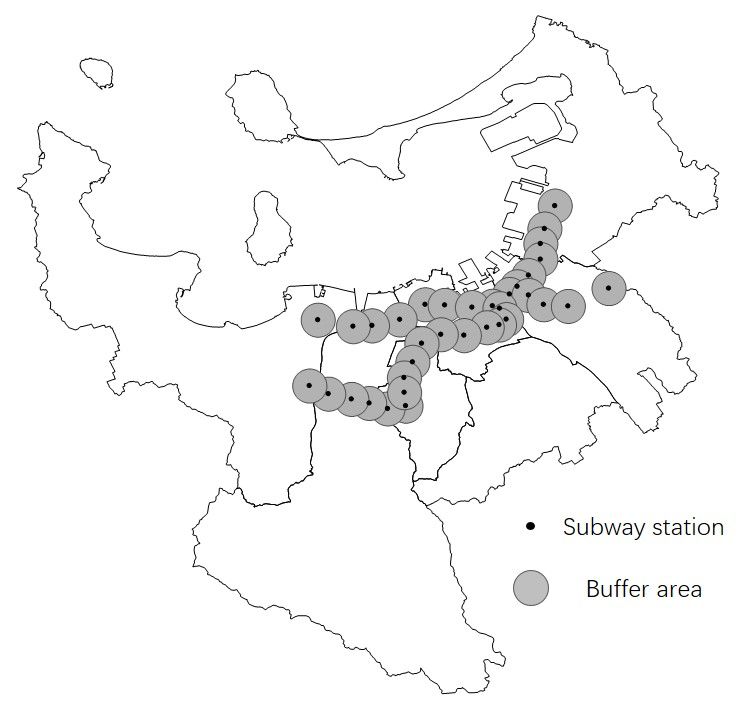
\includegraphics[width=\linewidth]{chapter3/BufferAreas}
	\caption{800-meter Circular buffer areas for 35 subway stations}
	\label{fig:chp3:BufferAreas}
\end{figure}

%
The land use data from Urban Planning Basic Survey is available every 5 years, to match the data period of transit ridership, the land use data on 2008 is used for analyzing characteristics of land use. The dataset of land use contains 23 types, which, however, are too many for analyzing the characteristics of land use in the case with only 35 stations. Moreover, most types of land use account for very little of the total building area, for which they are thought to have restricted influence on transit ridership. As a result, 9 types of land use, which have relatively larger building areas and commonly exist in all the catchment area of subway stations, are selected to analyze the characteristics of land use, the reserved items are listed in Figure \ref{fig:chp3:IndicatorSelection}.

%
\begin{figure}[htbp]
	\centering
	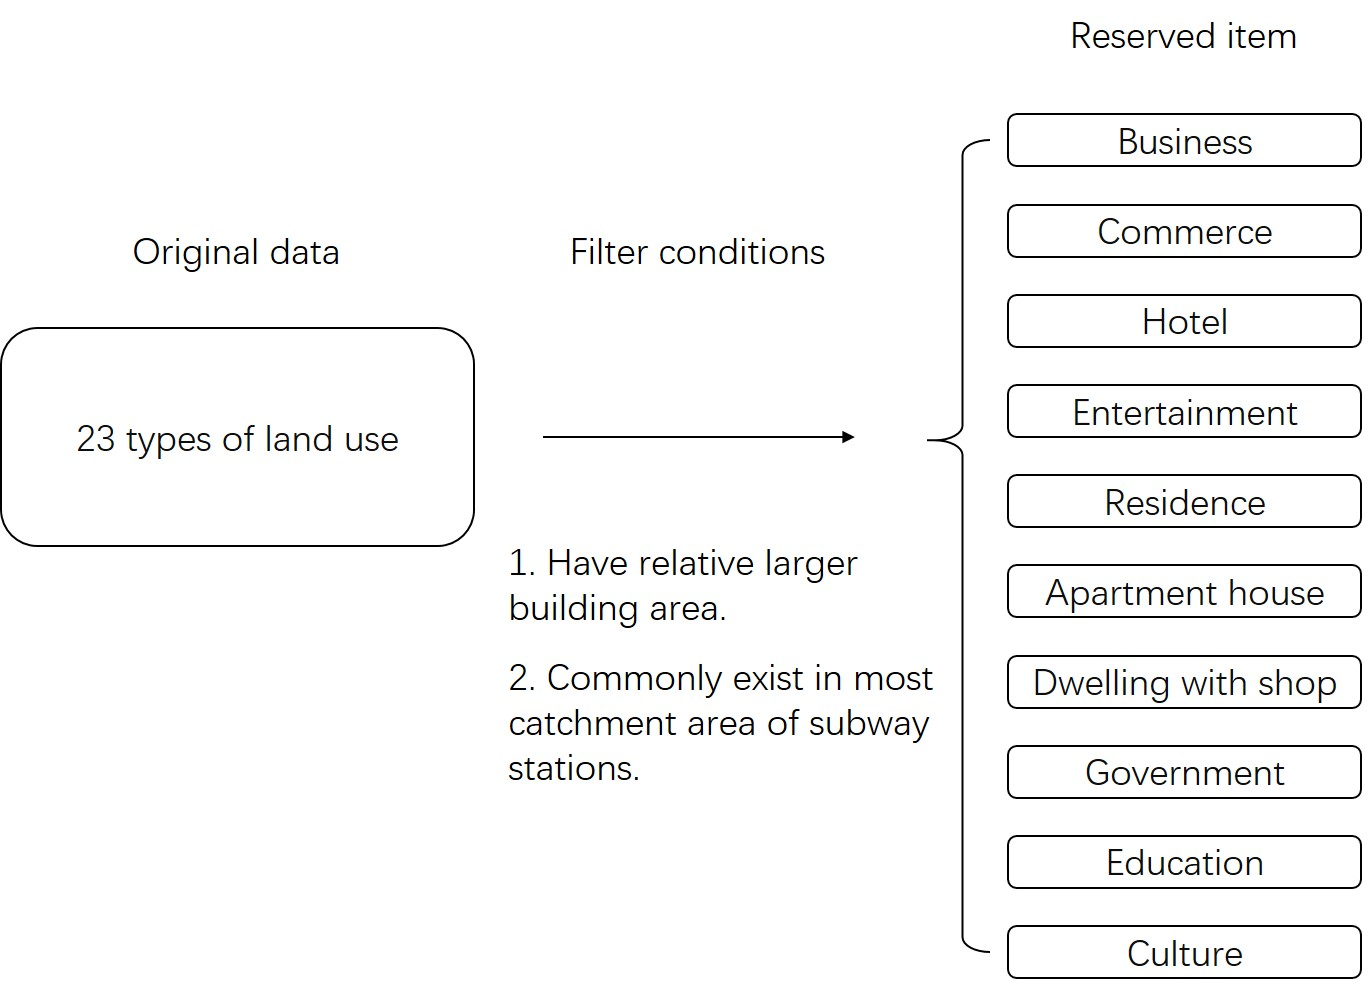
\includegraphics[width=\linewidth]{chapter3/IndicatorSelection}
	\caption{Flow of selecting indicators}
	\label{fig:chp3:IndicatorSelection}
\end{figure}

%
Through the initial screening, there are 10 indicators being selected. Nevertheless, restricted by the sample size of 35 stations, the 10 indicators are still too many to quantitatively examine the characteristics of land use. To further explore what these indicators are expressing, thus extracting valuable information, the correlation analysis is put forward to make clear of the relationship between indicators. The result of correlation analysis is shown in the Table \ref{tab:chp3:CorrelationAnalysis}. There are strong correlations between the 4 types of land use which are office, commerce, hotel, and entertainment. The type of dwelling with shop also has a strong correlation with that of office, commerce, and hotel, while the culture type of land use closely relates to the type of apartment and dwelling with shop.

%
\begin{sidewaystable}[htbp]
	\centering
	\caption{Correlation analysis for indicators}
	\label{tab:chp3:CorrelationAnalysis}
	\small
	\renewcommand{\arraystretch}{1.5} % 重设表间距
	\begin{tabular}{p{9em}|p{3em}<{\raggedleft}|p{3em}<{\raggedleft}|p{3em}<{\raggedleft}|p{3em}<{\raggedleft}|p{3em}<{\raggedleft}|p{3em}<{\raggedleft}|p{3em}<{\raggedleft}|p{3em}<{\raggedleft}|p{3em}<{\raggedleft}|p{3em}<{\raggedleft}}
		\Xhline{1.5pt}
		Indicator & 1 & 2 & 3 & 4 & 5 & 6 & 7 & 8 & 9 & 10 \\
		
		\Xhline{0.5pt}
		1. Business & 1.000 & \multicolumn{1}{r|}{\cellcolor[rgb]{ 0.8, 0.8, 0.8} 0.848} & \multicolumn{1}{r|}{\cellcolor[rgb]{ 0.8, 0.8, 0.8} 0.987} & \multicolumn{1}{r|}{\cellcolor[rgb]{ 0.8, 0.8, 0.8} 0.775} & -0.385 & 0.378  & \multicolumn{1}{r|}{\cellcolor[rgb]{ 0.8, 0.8, 0.8} 0.848} & 0.615  & 0.006  & 0.656 \\
		
		2. Commerce & \multicolumn{1}{r|}{\cellcolor[rgb]{ 0.8, 0.8, 0.8} 0.848} & 1.000 & {\cellcolor[rgb]{ 0.8, 0.8, 0.8} 0.828}  & \multicolumn{1}{r|}{\cellcolor[rgb]{ 0.8, 0.8, 0.8} 0.765} & -0.293 & 0.345  & \multicolumn{1}{r|}{\cellcolor[rgb]{ 0.8, 0.8, 0.8} 0.734} & 0.645  & 0.065  & 0.530 \\
		
		3. Hotel & \multicolumn{1}{r|}{\cellcolor[rgb]{ 0.8, 0.8, 0.8} 0.987} & \multicolumn{1}{r|}{\cellcolor[rgb]{ 0.8, 0.8, 0.8} 0.828} & 1.000 & \multicolumn{1}{r|}{\cellcolor[rgb]{ 0.8, 0.8, 0.8} 0.716} & -0.361 & 0.382  & \multicolumn{1}{r|}{\cellcolor[rgb]{ 0.8, 0.8, 0.8} 0.815} & 0.585  & 0.000  & 0.619 \\
		
		4. Entertainment & \multicolumn{1}{r|}{\cellcolor[rgb]{ 0.8, 0.8, 0.8} 0.775} & \multicolumn{1}{r|}{\cellcolor[rgb]{ 0.8, 0.8, 0.8} 0.765} & \multicolumn{1}{r|}{\cellcolor[rgb]{ 0.8, 0.8, 0.8} 0.716} & 1.000 & -0.322 & 0.281  & 0.663  & 0.439  & -0.018 & 0.552 \\
		
		5. Residence & -0.385 & -0.293 & -0.361 & -0.322 & 1.000 & 0.205  & -0.287 & -0.164 & -0.175 & -0.063 \\
		
		6. Apartment house & 0.378  & 0.345  & 0.382  & 0.281  & 0.205  & 1.000 & 0.649  & 0.408  &0.087  & \multicolumn{1}{r}{\cellcolor[rgb]{ 0.8, 0.8, 0.8} 0.729} \\
		
		7. Dwelling with shop & \multicolumn{1}{r|}{\cellcolor[rgb]{ 0.8, 0.8, 0.8} 0.848} & \multicolumn{1}{r|}{\cellcolor[rgb]{ 0.8, 0.8, 0.8} 0.734} & \multicolumn{1}{r|}{\cellcolor[rgb]{ 0.8, 0.8, 0.8} 0.815} & 0.663  & -0.287 & 0.649  & 1.000 & 0.641  & 0.038  & \multicolumn{1}{r}{\cellcolor[rgb]{ 0.8, 0.8, 0.8} 0.808} \\
		
		8. Government & 0.615  & 0.645  & 0.585  & 0.439  & -0.164 & 0.408  & 0.641  & 1.000 & 0.395  & 0.549 \\
		
		9. Education & 0.006  & 0.065  & 0.000  & -0.018 & -0.175 & 0.087  & 0.038  & 0.395  & 1.000 & -0.012 \\
		
		10. Culture & 0.656  & 0.530  & 0.619  & 0.552  & -.063 & \multicolumn{1}{r|}{\cellcolor[rgb]{ 0.8, 0.8, 0.8} 0.729} & \multicolumn{1}{r|}{\cellcolor[rgb]{ 0.8, 0.8, 0.8} 0.808} & 0.549  & -0.012 & 1.000 \\
		\Xhline{1.5pt}
	\end{tabular}%
\end{sidewaystable}%

\subsubsection{Factor analysis}
%
To deal with the strong collinearity among indicators, also to further make clear of the internal relationship, the exploratory factor analysis is introduced to reduce the dimension of the indicators, thus exploring the meanings that the indicators express. The factor analysis is a statistical method used to describe variability among observed, correlated variables in terms of a potentially lower number of unobserved variables, for which the factor analysis is usually used for dealing with the indicator set with strong collinearity. The procedure of factor analysis is as below.

%
\emph{1. KMO and Bartlett's Test}

%
The KMO measure of sampling adequacy reflect the correlation among all the indicators, referring to Table \ref{tab:chp3:KMOBartlettTest}. The test result of 0.756, which is greater than the suggested value of 0.7, means this indicator set has enough collinearity to conduct the factor analysis. As to the Bartlett’s Test, if the variables are independent to each other, the common factor cannot be extracted from it, and factor analysis cannot be applied. The Bartlett sphere test judges that if the correlation matrix is a unit matrix, the factor analysis method of each variable is invalid. The test results show that $Sig.<0.05$, which means that each variable has correlation and factor analysis is effective. 

% Table
\begin{table}[htbp]
	\centering
	\caption{KMO and Bartlett's Test}
	\label{tab:chp3:KMOBartlettTest}
	\small
	\renewcommand{\arraystretch}{1.25} % 重设表间距
	\begin{tabular}{p{16em}<{\centering}rr}
		\Xhline{1.5pt}
		\multicolumn{2}{c}{Kaiser-Meyer-Olkin Measure of Sampling Adequacy} & 0.756 \\
		\midrule
		
		\multirow{3}[0]{16em}{\centering{Bartlett's Test of Sphericity}} & \multicolumn{1}{r}{Chi-Square} & 346.086 \\
		& df & 45 \\
		& Sig. & 0.000 \\
		\Xhline{1.5pt}
	\end{tabular}%
\end{table}%

%
\emph{2. Factor extraction}

%
The factors are extracted using principal component method, Table \ref{tab:chp3:Communalities} lists the communalities of the indicators. As shown in this table, most information contained in the indicators can be explained by the extracted factors. Less information loss during the process of extracting factors means a good effect.

%
% Table generated by Excel2LaTeX from sheet 'Sheet2'
\begin{table}[htbp]
	\centering
	\caption{Communalities of each indicator}
	\label{tab:chp3:Communalities}
	\small
	\renewcommand{\arraystretch}{1.25} % 重设表间距
	\begin{tabular}{lrr}
		\Xhline{1.5pt}
		Indicator & Initial & Extraction \\
		\midrule
		
		Office & 1.000 & 0.943 \\
		Commerce & 1.000 & 0.799 \\
		Hotel & 1.000 & 0.890 \\
		Entertainment & 1.000 & 0.725 \\
		Residence & 1.000 & 0.710 \\
		Apartment house & 1.000 & 0.849 \\
		Dwelling with shop & 1.000 & 0.885 \\
		Government & 1.000 & 0.756 \\
		Education & 1.000 & 0.923 \\
		Culture & 1.000 & 0.811 \\
		\Xhline{1.5pt}
	\end{tabular}
\end{table}%

%
As a result, there are four factors with the eigenvalue greater than 1.00 being extracted, these four factors account for 82.90\% of all the variance. It means the three factors can explain most part of the original 10 indicators. The Table \ref{tab:chp3:TotalVarianceExplained} shows the total variance explained.

%
% Table generated by Excel2LaTeX from sheet 'Sheet2'
\begin{table}[htbp]
	\centering
	\caption{Total variance explained}
	\label{tab:chp3:TotalVarianceExplained}%
	\small
	\renewcommand{\arraystretch}{1.25} % 重设表间距
	\begin{tabular}{cccc}
		\Xhline{1.5pt}
		\multirow{2}[4]{*}{Component} & \multicolumn{3}{p{15em}}{Rotation Sums of Squared Loadings} \\
		\cmidrule{2-4}
		& Total & \% of Variance & Cumulative \% \\
		\midrule
		
		1 & 5.068 & 50.676 & 50.676 \\
		2 & 1.851 & 18.510 & 69.187 \\
		3 & 1.372 & 13.716 & 82.902 \\
		\Xhline{1.5pt}
	\end{tabular}%
\end{table}%

%
\emph{3. Factor naming and interpretation}

%
The rotated component matrix (Table \ref{tab:chp3:RotatedComponent}) shows the attribution of each indicators on the newly extracted factors. The three factors can be named and explained as follow, they are Office \& commerce, mixed-residence, education.

%
\begin{itemize}
	\item \textbf{Factor 1: Office \& commerce} \\
	This factor represents the land use mainly including office area, large commercial area, and some commercial supporting facilities.
	
	\item \textbf{Factor 2: Mixed residence} \\
	The indicators of apartment, residence, and culture mainly attribute to this factor, which can reflect the attribute of residence with supporting facilities.
	
	\item \textbf{Factor 3: Education} \\
	Except for the indicator of education, the indicator of government also attributes a large part of this factor. It means that the land use of education and government have a relatively strong correlation.
\end{itemize}

% Table
\begin{table}[htbp]
	\centering
	\caption{Rotated Component Matrix}
	\label{tab:chp3:RotatedComponent}%
	\small
	\renewcommand{\arraystretch}{1.25} % 重设表间距
	\begin{tabular}{lp{3em}<{\centering}p{3em}<{\centering}p{3em}<{\centering}}
		\Xhline{1.5pt}
		\multirow{2}[3]{*}{Indicator} & \multicolumn{3}{c}{Component} \\
		\cmidrule{2-4}
		& 1 & 2 & 3 \\
		\midrule
		
		Office & \cellcolor[rgb]{ 0.8,  0.8, 0.8} 0.962 & 0.122 & 0.060 \\
		Hotel & \cellcolor[rgb]{ 0.8,  0.8, 0.8} 0.934 & 0.123 & 0.050 \\
		Commerce & \cellcolor[rgb]{ 0.8,  0.8, 0.8} 0.878 & 0.105 & 0.131 \\
		Entertainment & \cellcolor[rgb]{ 0.8,  0.8, 0.8} 0.850 & 0.044 & -0.030 \\
		Dwelling with shop & \cellcolor[rgb]{ 0.8,  0.8, 0.8} 0.834 & 0.417 & 0.125 \\
		Apartment house & 0.301 & \cellcolor[rgb]{ 0.8,  0.8, 0.8} 0.860 & 0.134 \\
		Residence & -0.521 & \cellcolor[rgb]{ 0.8,  0.8, 0.8} 0.620 & -0.234 \\
		Education & -0.066 & -0.039 & \cellcolor[rgb]{ 0.8,  0.8, 0.8} 0.958 \\
		Culture & \cellcolor[rgb]{ 0.8,  0.8, 0.8} 0.627 & \cellcolor[rgb]{ 0.8,  0.8, 0.8} 0.644 & 0.057 \\
		Government & 0.570  & 0.305 & \cellcolor[rgb]{ 0.8,  0.8, 0.8} 0.582 \\
		\Xhline{1.5pt}
	\end{tabular}%
	\label{tab:addlabel}%
\end{table}%

%
\subsection{Classification of stations}
%
To further explore the characteristics of land use in terms of each station, the cluster analysis is used to classify all the 35 subway stations, and the characteristics are summarized respect to the classifications.

%
The indicators used for classifying the subway stations are selected on the base of correlation analysis and factor analysis conducted before. Although the indicator of office and commerce have a strong collinearity, the definitions and usage of them are quite different, therefore, both of the two indicators are used in cluster analysis. Also with the consideration of the internal correlations shown in Table \ref{tab:chp3:CorrelationAnalysis}, the indicators with relatively high independence are selected. At last, there are 4 indicators of land use being selected for classification, they are office, commerce, residence, education, adding to one more indicator of population density is selected to describe the characteristic of density.

%
As to the procedure of cluster analysis, the cluster method is Ward Method, the measurement of interval uses the Squared Euclidean Distance, the data is standardized into 0.00-1.00 range. The 34 of all the 35 subway stations fall into 5 types, while the No.7 station located in the Fukuoka airport differs from the others. The 5 types are: low-density residence (9 stations), high-density residence (9 stations), education (6 stations), downtown commerce (5 stations), and office (5 stations) respectively. The result of classification is in the Figure \ref{fig:chp3:StationClassification}, the right part of this Table is the pie chart of land use which shows the proportion of land use. The description of each type of stations is given below. 

%
\begin{figure}[htbp]
	\centering
	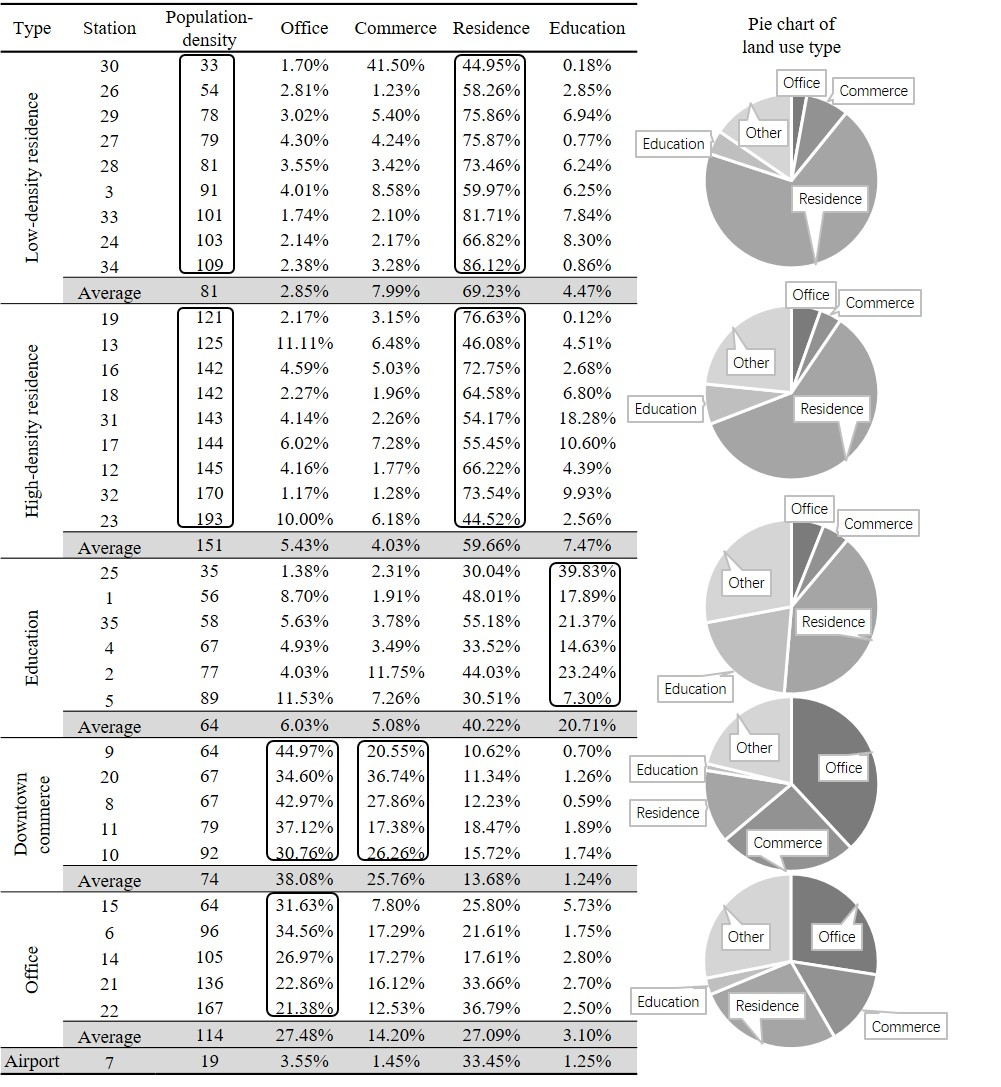
\includegraphics[width=\linewidth]{chapter3/StationClassification}
	\caption{Classification of stations in terms of land use}
	\label{fig:chp3:StationClassification}
\end{figure}

%
\begin{itemize}
	\item \textbf{Characteristics of low-density residence type} \\
	This type has 9 stations with the characteristics of high proportion of residence, and low population-density, very few office and commerce.
	
	\item \textbf{Characteristics of High-density residence type} \\
	The proportion of each land use in high-density residence is similar with that in low-density residence type, but population-density is much higher than other types.
	
	\item \textbf{Characteristics of education type} \\
	This type has 6 stations, they are located in the vicinity of colleges and universities, and the service population is mainly students and nearby residents.
	
	\item \textbf{Characteristics of downtown commerce type} \\
	The type of downtown commerce includes 5 stations, which constituted the CBD area of Fukuoka. These stations have the highest proportion of office and commerce, while proportion of residence is the lowest and population density is relatively lower.
	
	\item \textbf{Characteristics of office type} \\
	This type includes 5 stations, of which the main land use is office. These stations mainly distribute around the CBD area, mixed land use is one of the main characteristics.
\end{itemize}

%
The No.7 Kukou station, which locates at Fukuoka airport, is different from the other 5 types of stations, the main component of land use is transportation facilities. From the view of land use, reflecting into the result of classification, the No.7 station does not belong to any type of stations.

%
\section{Exploration on the relationship between land use and transit ridership}
\subsection{General relationship between land use and transit ridership}
%
The data of land use is conducted every 5 years, while the data of subway transit ridership is annual. The 2008 data included in both data is used to analyze the relationship between subway transit ridership and land use.

%
According to the classification result (refer to \ref{fig:chp3:StationClassification}), adding to the average transit ridership of each type of station, as shown in the Table \ref{tab:chp3:ClassificationCharacteristics}, the subway transit ridership varies a lot in different types of land use. The station of low-density residence type has an average transit ridership of only 3,416, while that of high-density residence type has 15,633 on average. The downtown commerce type has the highest average transit ridership of 52,300, while that in office type is only 11,038, even though similar with the type of downtown commerce the office type has a high proportion of land use in office and commerce. The proportions of office and commerce in education type are similar with that in the two residence types, but from which the average transit ridership is quite different.

% Table
\begin{table}[htbp]
	\centering
	\caption{Characteristic of each classification}
	\label{tab:chp3:ClassificationCharacteristics}
	\small
	\renewcommand{\arraystretch}{1.25} % 重设表间距
	\begin{tabular}{lp{4em}<{\raggedleft}p{4em}<{\raggedleft}p{4em}<{\raggedleft}p{4em}<{\raggedleft}p{4em}<{\raggedleft}}
		\Xhline{1.5pt}
		Type & Office & Commerce & Residence & Education & Transit ridership \\
		\midrule
		
		Low-density residence & 2.85\% & 7.99\% & 69.23\% & 4.47\% & 3416 \\
		High-density residence & 5.43\% & 4.03\% & 59.66\% & 7.47\% & 15633 \\
		Education & 6.03\% & 5.08\% & 40.22\% & 20.71\% & 7391 \\
		Downtown commerce & 38.08\% & 25.76\% & 13.68\% & 1.24\% & 52300 \\
		Office & 27.48\% & 14.20\% & 27.09\% & 3.10\% & 11038 \\
		\Xhline{1.5pt}
	\end{tabular}
\end{table}

%
According to the classification result of both subway transit ridership and land use around the stations, the cross table is shown in the Figure \ref{tab:chp3:CrossTable} below. All the stations belonging to low-density residence type have small-scale of transit ridership, which is under 10,000 per day. Both the two hub stations belonging to the downtown commerce type located in the CBD area of Fukuoka. Overall, it can be inferred from this table that the area with lower density either in population or building has a lower demand in using rail transit; besides the high density in population and building, hub stations should also have particularities in location and function. 

% Table
\begin{table}[htbp]
	\centering
	\caption{Cross tabulation of land use and transit ridership}
	\label{tab:chp3:CrossTable}
	\small
	\renewcommand{\arraystretch}{1.25} % 重设表间距
	\begin{tabular}{lp{3em}<{\raggedleft}p{3em}<{\raggedleft}p{3em}<{\raggedleft}p{3em}<{\raggedleft}}
		\Xhline{1.5pt}
		Type & Hub & Large-scale & Medium-scale & Small-scale \\
		\midrule
		
		Low-density residence & 0 & 0 & 0 & 9 \\
		High-density residence & 0 & 2 & 4 & 3 \\
		Education & 0 & 0 & 1 & 5 \\
		Downtown commerce & 2 & 1 & 2 & 0 \\
		Office & 0 & 0 & 3 & 2 \\
		\Xhline{1.5pt}
	\end{tabular}
\end{table}

%
Through the characteristics analysis of subway transit ridership and land use, the general trend of the relationship between them can be understood. However, the conclusion obtained from the trend analysis cannot be fully trusted due to the lack of quantitative analysis, also, how the factor land use can influence transit ridership is still not clear.

\subsection{Statistical relationship of land use and transit ridership}
%
The quantification method \uppercase\expandafter{\romannumeral1} is introduced to further explore the influence of each factor on the transit ridership. Different from regression model, the quantification method \uppercase\expandafter{\romannumeral1} converts the continuous independent variables into categorical variables thus investigating the correlation between categorical independent variables and the continuous dependent variable. This method is thought suitable to do the exploratory analysis on the data for the first time due to the procedure of discretizing the continuous independent variables. This discretization can partly reduce the deviation caused by the uneven distribution of the sample in the whole.

%
The quantification method \uppercase\expandafter{\romannumeral1} can be viewed as an improvement of regression model which is used for dealing with the exploratory analysis at the beginning. Therefore, in the process of selecting explaining indicators, the indicators with strong collinearity should be excluded. Referring to the Table \ref{tab:chp3:CorrelationAnalysis}, the indicators of office, residence, education, and government have less collinearity. Notably, the indicators of office and commerce have strong collinearity, but either of the two indicators accounts for a large part in total, for which they should not be easily ignored. In order to reserve more information, a new indicator named commerce \& office which represents the sum of commerce and office building area is proposed. Coupled with the indicator of population density, there are 5 influencing indicators selected as the independent variables. The division of continuous variables are determined based on the Squared Euclidean distance between groups. Both the transit ridership and growth rate of transit ridership are estimated using the 5 indicators of population density, commercial \& office, residence, education, and government. The result is shown as Table \ref{tab:chp3:QM1TransitRidership} and Table \ref{tab:chp3:QM1GrowthRate}.

%
As the results, the coefficients of determination with the value of 0.513 and 0.537 in both models respectively are not satisfactory. However, the results are not for predicting the transit ridership in the future but for exploring the influence of land use on the transit ridership. In view of this, the results are thought to have a certain referential value. 

%
As to the result of influence on the transit ridership, the commerce \& office contributes most of the variation in the transit ridership, which means that the commerce \& office plays important role in explaining the transit ridership. The building area of education has the weakest influence, while even building area of government is much smaller than that of education, the indicator of government contributes more to the variation in transit ridership. 

% Table
\begin{table}[htbp]
	\centering
	\caption{Results of quantification method \uppercase\expandafter{\romannumeral1} on transit ridership}
	\label{tab:chp3:QM1TransitRidership}
	\small
	\renewcommand{\arraystretch}{1.25} % 重设表间距	
	\begin{tabular}{p{8em}rp{4em}<{\raggedleft}p{4em}<{\raggedleft}p{4em}<{\centering}}
		\Xhline{1.5pt}	
		Factor category & Category & Number & Score & \multirow{1}[1]{4em}{Range} \\
		\midrule
		
		\multirow{5}[0]{8em}{population density \\ (person/ha)} & 0-40  & 3 & 4644 & \multirow{5}[0]{4em}{13004 \\ 13.84\%} \\
		& 40-80 & 13 & 2283 & \\
		& 80-120 & 8 & 164 &  \\
		& 120-160 & 8 & -2481 &  \\
		& 160- & 3 & -8360 &  \\
		\midrule
		
		\multirow{4}[0]{8em}{Commerce \& Office \\ ($m^2$)} & 0-100,000 & 16 & -6249 & \multirow{4}[0]{4em}{43288 \\ 46.07\%} \\
		& 100,000-400,000 & 9 & -6617 &\\
		& 400,000-1,000,000 & 5 & -4765 & \\
		& 1,000,000- & 5 & 36671 & \\
		\midrule
		
		\multirow{3}[0]{8em}{Residence \\ ($m^2$)} & 0-300,000 & \multicolumn{1}{r}{4} & -1450 & \multirow{3}[0]{4em}{16240 \\ 17.28\%} \\
		& 300,000-800,000 & 20 & -5575 & \\
		& 800,000- & 11 & 10664 & \\
		\midrule
		
		\multirow{3}[0]{8em}{Government \\ ($m^2$)} & 0-1,000 & 13 & -2957 & \multirow{3}[0]{4em}{12267 \\ 13.06\%} \\
		& 1,000-10,000 & 9 & -5501 & \\
		& 10,000- & 13 & 6766 & \\
		\midrule
				
		\multirow{4}[0]{8em}{Education \\ ($m^2$)} & 0-10,000 & 5 & 4842 & \multirow{4}[0]{4em}{9159 \\ 9.75\%}\\
		& 10,000-50,000 & 11 & 993 & \\
		& 50,000-100,000 & 11 & -4317 & \\
		& 100,000- & 8 & 1544 & \\
		\Xhline{0.5pt}
				
		\multicolumn{2}{c|}{Independent variable} & \multicolumn{2}{c}{Sample size} & 35 \\
		\multicolumn{2}{c|}{Transit ridership} & \multicolumn{2}{c}{Coefficient of determination} & 0.513 \\
		\Xhline{1.5pt}
	\end{tabular}%
\end{table}%

% Table
\begin{table}[htbp]
	\centering
	\caption{Results of quantification method \uppercase\expandafter{\romannumeral1} on growth rate of transit ridership}
	\label{tab:chp3:QM1GrowthRate}
	\small
	\renewcommand{\arraystretch}{1.25} % 重设表间距	
	\begin{tabular}{p{8em}rp{4em}<{\raggedleft}p{4em}<{\raggedleft}p{4em}<{\centering}}
		\Xhline{1.5pt}	
		Factor category & Category & Number & Score & \multirow{1}[1]{4em}{Range} \\
		\midrule
		
		\multirow{5}[0]{8em}{population density \\ (person/ha)} & 0-40  & 3 & 0.0155 & \multirow{5}[0]{4em}{0.0265 \\ 28.44\%} \\
		& 40-80 & 13 & 0.0020 & \\
		& 80-120 & 8 & -0.0001 & \\
		& 120-160 & 8 & -0.0110 & \\
		& 160- & 3 & 0.0056 & \\
		\midrule
		
		\multirow{4}[0]{8em}{Commerce \& Office \\ ($m^2$)} & 0-100,000 & 16 & -0.0016 & \multirow{4}[0]{4em}{0.0097 \\ 10.44\%} \\
		& 100,000-400,000 & 9 & 0.0006 & \\
		& 400,000-1,000,000 & 5 & 0.0069 & \\
		& 1,000,000- & 5 & -0.0028 & \\
		\midrule
		
		\multirow{3}[0]{8em}{Residence \\ ($m^2$)} & 0-300,000 & \multicolumn{1}{r}{4} & -0.0183 & \multirow{3}[0]{4em}{0.0226 \\ 24.31\%} \\
		& 300,000-800,000 & 20 & 0.0043 & \\
		& 800,000- & 11 & -0.0012 & \\
		\midrule
		
		\multirow{3}[0]{8em}{Government \\ ($m^2$)} & 0-1,000 & 13 & 0.0111 & \multirow{3}[0]{4em}{0.0228 \\ 24.54\%} \\
		& 1,000-10,000 & 9 & 0.0008 & \\
		& 10,000- & 13 & -0.0117 & \\
		\midrule
		
		\multirow{4}[0]{8em}{Education \\ ($m^2$)} & 0-10,000 & 5 & -0.0078 & \multirow{4}[0]{4em}{0.0114 \\ 12.27\%}\\
		& 10,000-50,000 & 11 & -0.0025 & \\
		& 50,000-100,000 & 11 & 0.0034 & \\
		& 100,000- & 8 & 0.0036 & \\
		\Xhline{0.5pt}
		
		\multicolumn{2}{c|}{Independent variable} & \multicolumn{2}{c}{Sample size} & 35 \\
		\multicolumn{2}{c|}{Growth rate of transit ridership} & \multicolumn{2}{c}{Coefficient of determination} & 0.537 \\
		\Xhline{1.5pt}
	\end{tabular}
\end{table}


%
The same indicator set is also used for estimating the influence on the growth rate of transit ridership (Table \ref{tab:chp3:QM1GrowthRate}), as a result, the coefficient of determination is a little higher than that of transit ridership. The indicator of commerce \& office explains only 10\% of the total variation in growth rate, while it accounts for almost 50\% in the case of transit ridership. This result shows that the driving force of transit ridership and of transit ridership growth rate is different. The factor of population and residents play the key roles in promoting the use of subway.

%
\section{Conclusion}
%
This study investigated the variation of subway transit passengers from 2005 to 2014, and then analyzed the types of land use around the stations. On the base of understanding the characteristics of transit ridership and land use, the relationship between them was also estimated. The 35 subway stations were classified into 5 types with typical characteristics in terms of land use. The transit ridership of each type of stations showed significant differences. The results from quantification method \uppercase\expandafter{\romannumeral1} showed the quantitative relationship between transit ridership and land use. Even though the accuracy of results was not enough to make a prediction, it provided references for selecting more valid indicator to make a prediction in the future research.

%
The major finding of this study can be summarized as follows. 

%
\begin{itemize}
	\item From the comprehensive description of the study case and the investigation on the transit ridership, it can be known that the subway transit ridership is still increasing at present, but it probably turns to decrease within the near future. 
	
	\item The subway line 3 has a greater potential for growth in transit ridership. Even though the transit ridership also the population and building density are still lower at present, the stations in subway line 3 are under rapid developing.
	
	\item The spatial variation in transit ridership shows the characteristics of central aggregation. The hub stations with higher transit ridership near to the downtown area have a higher growth rate in transit ridership.
	
	\item According to the classification of stations in terms of land use, different types of stations have quite different scales on the transit ridership.
	
	\item The same indicators of land use have different effects on transit ridership and the growth rate of transit ridership.
\end{itemize}

%
This study is the first step to explain the influencing factors on rail transit ridership, which aims to give a comprehensive description of the research objects also provide references for further explaining transit ridership. Based on the understanding of the insufficiencies in this study, some recommendations are given for the next research.

%
\begin{itemize}
	\item The determination of catchment area needs more investigation. Since the 800-meter circle catchment does not consider the differences in the form of the road network, the same 800 meters catchment area may represent different walking distance reflecting on the real road network.
	
	\item The selection of indicators explaining the transit ridership needs more exploration. The other categories of indicators about such as facilities, socio-economic, and urban design should also have influence on the transit ridership.
	
	\item The selection and usage of estimation model need more investigation. The issue of transit ridership is not only a simple regression problem, but it also relates to the location of stations. A model which is suitable for spatial analysis may be better than an ordinary regression model. 
	
	\item The approach of dealing with small sample case should be considered. Statistical analysis needs a certain sample size, otherwise, it cannot say the estimation result is credible. The problem led by small sample also reflects on the procedure of selecting the valid explanatory variables. 
\end{itemize}


% reference
\clearpage % 新起一页
\bibliographystyle{apacite}
% \bibliographystyle{IEEEtran}
\bibliography{ref}

\chapter{Catchment Area and Walking Preference}
\markright{CHAPTER 4}

% 待修正
\section{Introduction}
% 略微重复一点第一章内容,说明我要做的背景
At present, the 800m (half-mile) walking distance has been widely accepted as a principal reference of the catchment area for the planning of Transit-Oriented Development (TOD) \cite{kuby2004factors,gutierrez2011transit,cardozo2012application,zhao2013influences}. Planners and researchers also use rail transit catchment areas to make prediction of ridership. However, this 800m walking distance is loosely obtained from the sampling survey by asking how far people are willing to walk to rail transit stations, and the same reasoning has been used to justify other rail transit catchment areas and even in different cities and countries. As to passengers, the acceptable walking distance/duration should not only relate to the features of the built environment such as the scale of stations and the functions of the buildings around stations, but also relate to the features of passengers' individual characteristics, such as occupations and trip purposes.

% 一个类比
Rail transit provides a cheaper and environment-friendly way of transportation to passengers. Like any other service and commodities, it needs to face the market and should be transacted at the cost acceptable to consumers. As a result, the distribution of transaction cost can reflect the consumption-ability of consumers in the market. Obviously, it is important for rail transit operators to know how much the cost that consumers are willing to pay, based on which thereby making rail transit more attractive. But a little different from general service and commodities, for passengers, the cost refers to the convenience rather than the fare, because the cheap enough fare is already not the important element for passengers to decide whether using rail transit while the walking duration to stations become the important determinant.

% 转换回轨道交通乘客时的选择问题
In the case of rail transit, before a potential passenger makes the decision of walking to a station, the expected walking duration, which is the "price" for this potential passenger, is just the reflection of the distance between departures and stations; while if this expected walking duration can be accepted by this potential passenger, this trip will happen and be surveyed. Based on the analogy given before, it's easy to think of that people with different individual characteristics generally should have different willingness towards walking duration to stations, and the surveyed walking durations can be viewed as the transaction price which have been accepted by passengers. It follows that the willingness of using rail transit will increase if the expected walking duration is less than that of acceptant range, otherwise, the willingness will decrease, which reflected in the survey data will be that the records with shorter walking duration are more than that with longer walking duration. 

% Introduction的总结
As interpreted above, although the walking duration just presents the distance between departures and stations, it should have relevance with individual characteristics. Thereby, this study uses Fukuoka, Japan, as the case to explore this relevance, trying to explore how long passengers with have different individual characteristics are willing to take for walking to stations. The sample mainly includes people's individual characteristics and trip chain information, for example gender, age, occupation, departures, destinations and travel time. This paper is constructed as follow: section two reviews the previous research from the factor of walking duration and the influencing factors two parts;  section three describes the data for Fukuoka, and presents methods and necessary assumptions; section four and five give the process of analysis; section six discusses the results and draws conclusions. 

%
\section{Review}
This section reviews the literature on the issue of walking duration/distance to rail transit stations, some problems that are still not well addressed are summarized. The review is arranged into two parts, which are the disposal of the variable of walking duration/distance, and the effect of influencing factors.

%
For the walking duration/distance, which is the research object in this study, there is always a difficult point in obtaining the accuracy walking duration/distance by questionnaire because of the discrepancy between perceived values and objective values. Also, the observed walking duration/distance is not the reflection of how long people are willing to spend on walking to rail transit stations, but only the walking duration/distance between departures and stations. For this problem, some studies chose a different perspective trying to explain the walking duration/distance by introducing a threshold of walking duration \cite{besser2005walking,mccormack2008objective}. They examined the differences in the distribution of influencing factors in terms of the specific threshold of walking duration. Indeed, using a threshold can decrease the discrepancy between observation and reality in some extent, but this disposal also brought some new problems in, for example, it may lead to a great loss of information in the raw data, and it is also difficult to decide the threshold of walking duration/distance.

%
Moreover, another point for this issue is whether to choose walking distance or walking duration as the threshold. To date, there are a lot of studies working on the relationship between walking distance and passengers' individual characteristics, some of them argued that an individual has a limited amount of time spending on traveling during a day, people tend to accept further walking distance as the speed of travel increases \cite{marchetti1994anthropological,larsen2010beyond}. With this reasoning it is easy to think of that passengers with the same individual characteristics may have the similar willingness of walking duration, but they generally have different willingness of walking distance due to different travel speed. This is also the reason why this study chooses the walking duration as the research object.

%
Among the influencing factors for walking durations, passengers' individual characteristics are generally thought to be the key that can affect walking distance \cite{besser2005walking,weinstein2008far,krygsman2004multimodal,yang2012walking,daniels2013explaining,guerra2012half}, whereas, there are few studies having clearly verified the relationship between individual characteristics and walking distance/duration, even there is a study suggesting the walking distance should not be viewed as a function of socio-demographic characteristics \cite{krygsman2004multimodal}. Several studies have confirmed the role of travel purposes in determining walking distance, the commute trip showed particularity from the other purposes, people with the purpose of commute tend to walk a longer distance to rail transit stations \cite{larsen2010beyond}. However, the definite relationship between trip purposes and walking distance is still unclear. The situation is the same with other categories of factors, such as the factors of transportation environment, land use, and willingness of passengers \cite{guerra2012half,krygsman2004multimodal,weinstein2008far}. The only thing that has been confirmed to date is that the walking distance/duration can be influenced by some specific kinds of factors, such as socio-demographic characteristics, trip purposes, and built-environment, but the problem is how and to what degree the walking distance/duration can be influenced.

%
It may be because of the problems in the disposal of walking distance/duration or the selection of influencing factors, most of the existing studies did not find the significant relevance between the walking distance/duration and the influencing factors. The studies working on the qualitative description for the distribution of walking distance accounted for the majority although some of the existing studies attempted regression model on this issue, the expected results were not obtained. To avoid the problems mentioned in the review, this study uses the thresholds of walking duration as the research object; for any given threshold of walking duration, the respondent who gives the answer greater than the given threshold can be viewed as this respondent can accept this threshold of walking duration; the surveyed walking duration is the reflection of passengers' willingness for using rail transit. For the analytical method, since various types of regression model has been verified unsuitable for this issue, instead of finding the linear relevance between dependent and independent variables, this study introduces the approach of machine learning into this issue, and try to explain the relevance between walking durations and individual characteristics from the view of probability.

%
\section{Data}
%
\subsection{Case introduction}
The study case of Fukuoka is the sixth largest city in Japan which has the population of more than 1.5 million. The dataset is the Northern Kyushu Area Person Trip, which is conducted about every 12 years, the latest available data is from the 4th survey surveyed by the year of 2005, and the 5th survey is already in preparation from September 2017. Figure \ref{fig:chp4:StationDistribution} shows the research area and the distribution of rail transit stations. By the year of 2005 (the 4th Northern Kyushu Area Person Trip Survey was conducted), there are more than 70 stations located within the city area of Fukuoka, of which the number of JR Kyushu station is 27, Fukuoka Subway station is 35, and West Japan Railway station is 16. Now some new rail transit lines and stations are still under planning and construction. According to the “Survey on the current state of public transportation” published by the Ministry of Land, Infrastructure, Transport and Tourism of Japan, the rail transit system in Fukuoka carries a daily average of more than 0.4 million passengers by 2015, accounting for more than 20\% in total motorized travel. Although the rail transit system of Fukuoka is still not a large-scale one at now, it has been playing a crucial role in people's daily travel.

% Figure 1
\begin{figure}[htbp]
	\centering
	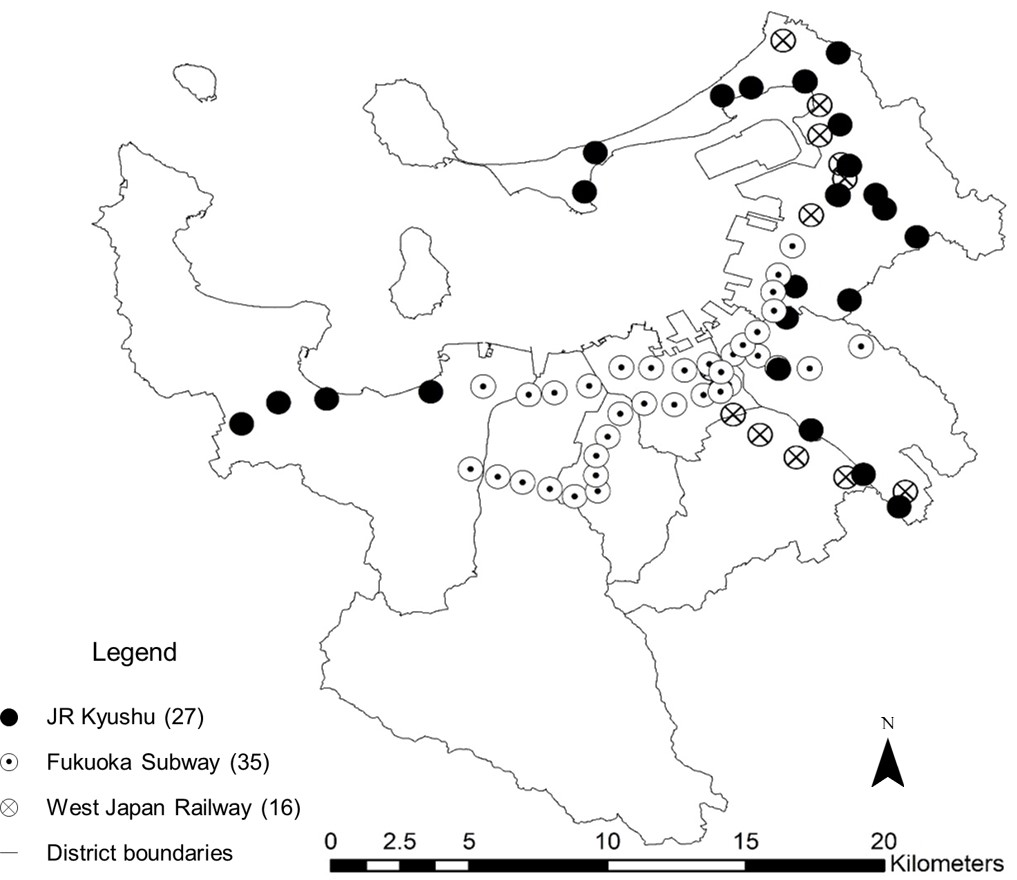
\includegraphics[width=0.8\linewidth]{chp4StationDistribution}
	\caption{Distribution of Transit Stations}
	\label{fig:chp4:StationDistribution}
\end{figure}

%
\subsection{Data description}
The main purpose of person trip survey is to know the travel trends, thus making a better living environment and providing support for traffic planning. The original data covered the range of all the main cities in Northern Kyushu Area, which has more than 483,000 records of trip chaining behavior. The available data in this study mainly includes trip chaining behavior and socio-demographic characteristics, as shown in the Table \ref{tab:chp4:Data}.

% Table 1
\begin{table}[htbp]
	\centering
	\caption{Available Data Contents}
	\label{tab:chp4:Data}
	\renewcommand{\arraystretch}{1.25} % 重设表间距
	
	\begin{tabular}{cc}
		\Xhline{1.5pt}
		Category                      & Feature\\
		\midrule
		\multirow{7}[0]{*}{Trip chaining behavior} 
		& Departure location \\
		& Departure time \\
		& Destination location \\
		& Arrival time \\
		& Transport modes \\
		& Time spent for each mode \\
		& Location of bus stop or rail transit station \\
		\Xhline{0.5pt}
		
		\multirow{6}[0]{*}{Socio-demographic attributes}
		& Age \\
		& Sex \\
		& Occupation \\
		& Trip purpose \\
		& Vehicle/License holding \\
		& Address \\
		\Xhline{1.5pt}
	\end{tabular}
\end{table}

%
To analyze the walking duration between departures and rail transit stations in Fukuoka, the first step is to extract the valid records of rail transit trip within the city area of Fukuoka from over 480,000 records in the dataset. The procedure of extracting the valid data is divided into 3 steps. Firstly, extracting all the person trip data that surveyed within the city area of Fukuoka; secondly, selecting the trip chaining behavior which contains the rail transit mode; thirdly, filtering the invalid data that with null value or abnormal value. The procedure of data cleaning is shown in Figure \ref{fig:chp4:DataCleaning}, at last the valid dataset is reduced to a size of 4254 trips.

% Figure 2
\begin{figure}[htbp]
	\centering
	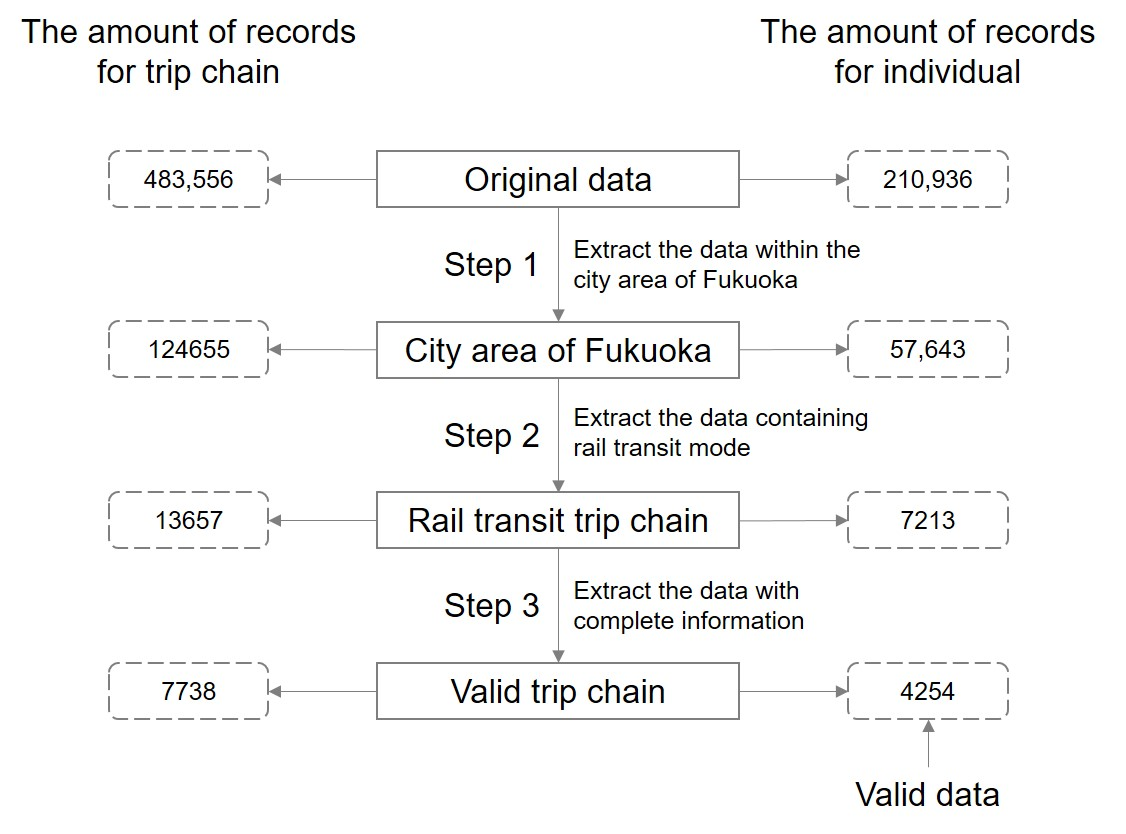
\includegraphics[width=0.9\linewidth]{chp4DataCleaning}
	\caption{Process of Data Cleaning}
	\label{fig:chp4:DataCleaning}
\end{figure}

%
Figure \ref{fig:chp4:AgeDistribution} shows the age distribution for walking trips to rail transit stations based on the finally valid dataset. The passengers aged from 25 to 55 account for the majority of the whole passengers, while schoolchildren aged under 15 rarely take rail transit. The distribution graph does not show significant peak values at any specific age group. Figure \ref{fig:chp4:DurationDistribution} shows the distribution of real walking durations to stations, it has a mean value of 8.32, and the standard deviation is 2. Notably, there are several peak values at the time of 5 multiples. It is speculated that the peak values may be caused by deviation occurred in the investigation. Since people's feeling about the specific time or number is inaccurate, they are inclined to reply a loose answer when they are asked some questions about the details of walking duration. This inclination will count some of the real walking duration that is near to 5 multiples as the 5 multiples and finally expressed in the result of investigation. Despite the bias between survey and reality, as the second assumption proposed before, passengers are viewed that they can accept the walking duration what they answered, therefore, the peak values are thought available in this study.

% Figure 3
\begin{figure}[htbp]
	\centering
	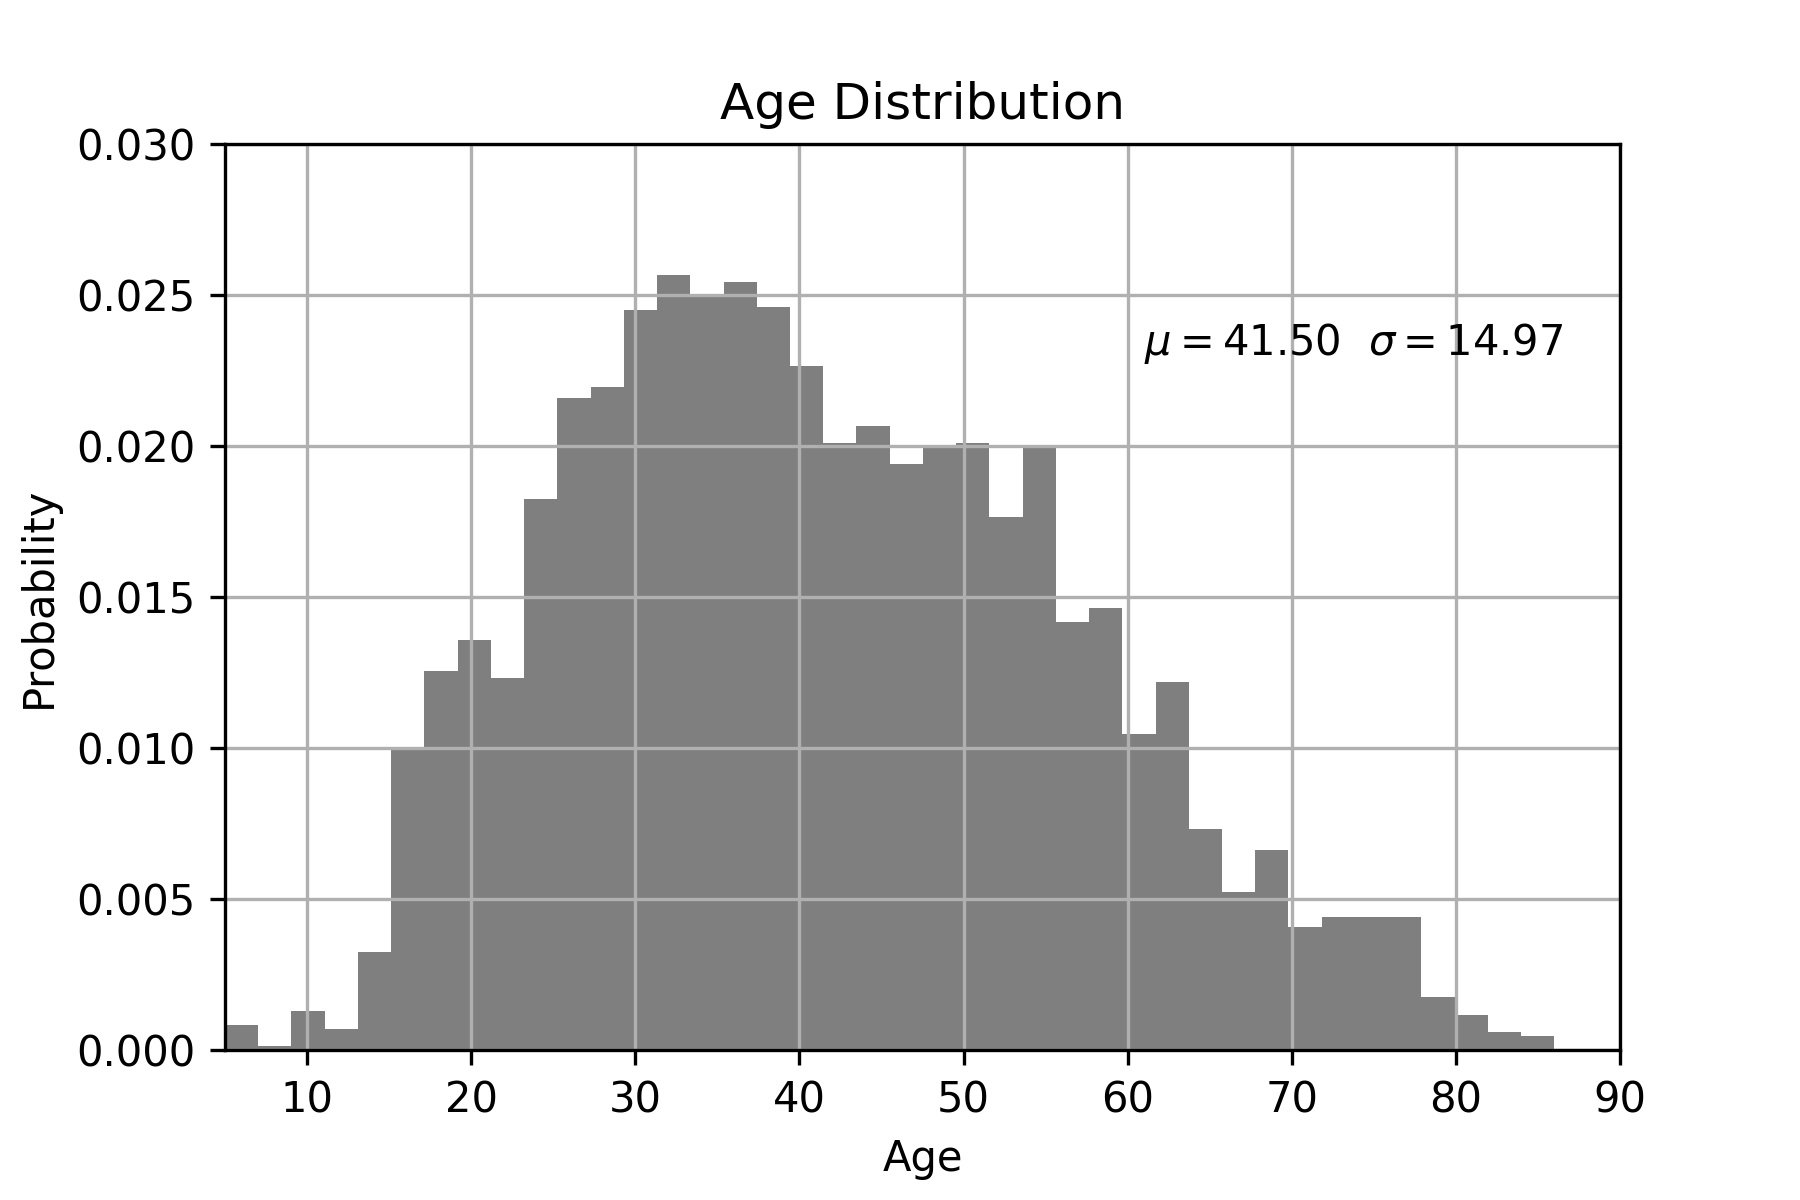
\includegraphics[width=\linewidth]{chp4AgeDistribution}
	\caption{The Age Distribution of Passengers}
	\label{fig:chp4:AgeDistribution}
\end{figure}

% Figure 4
\begin{figure}[htbp]
	\centering
	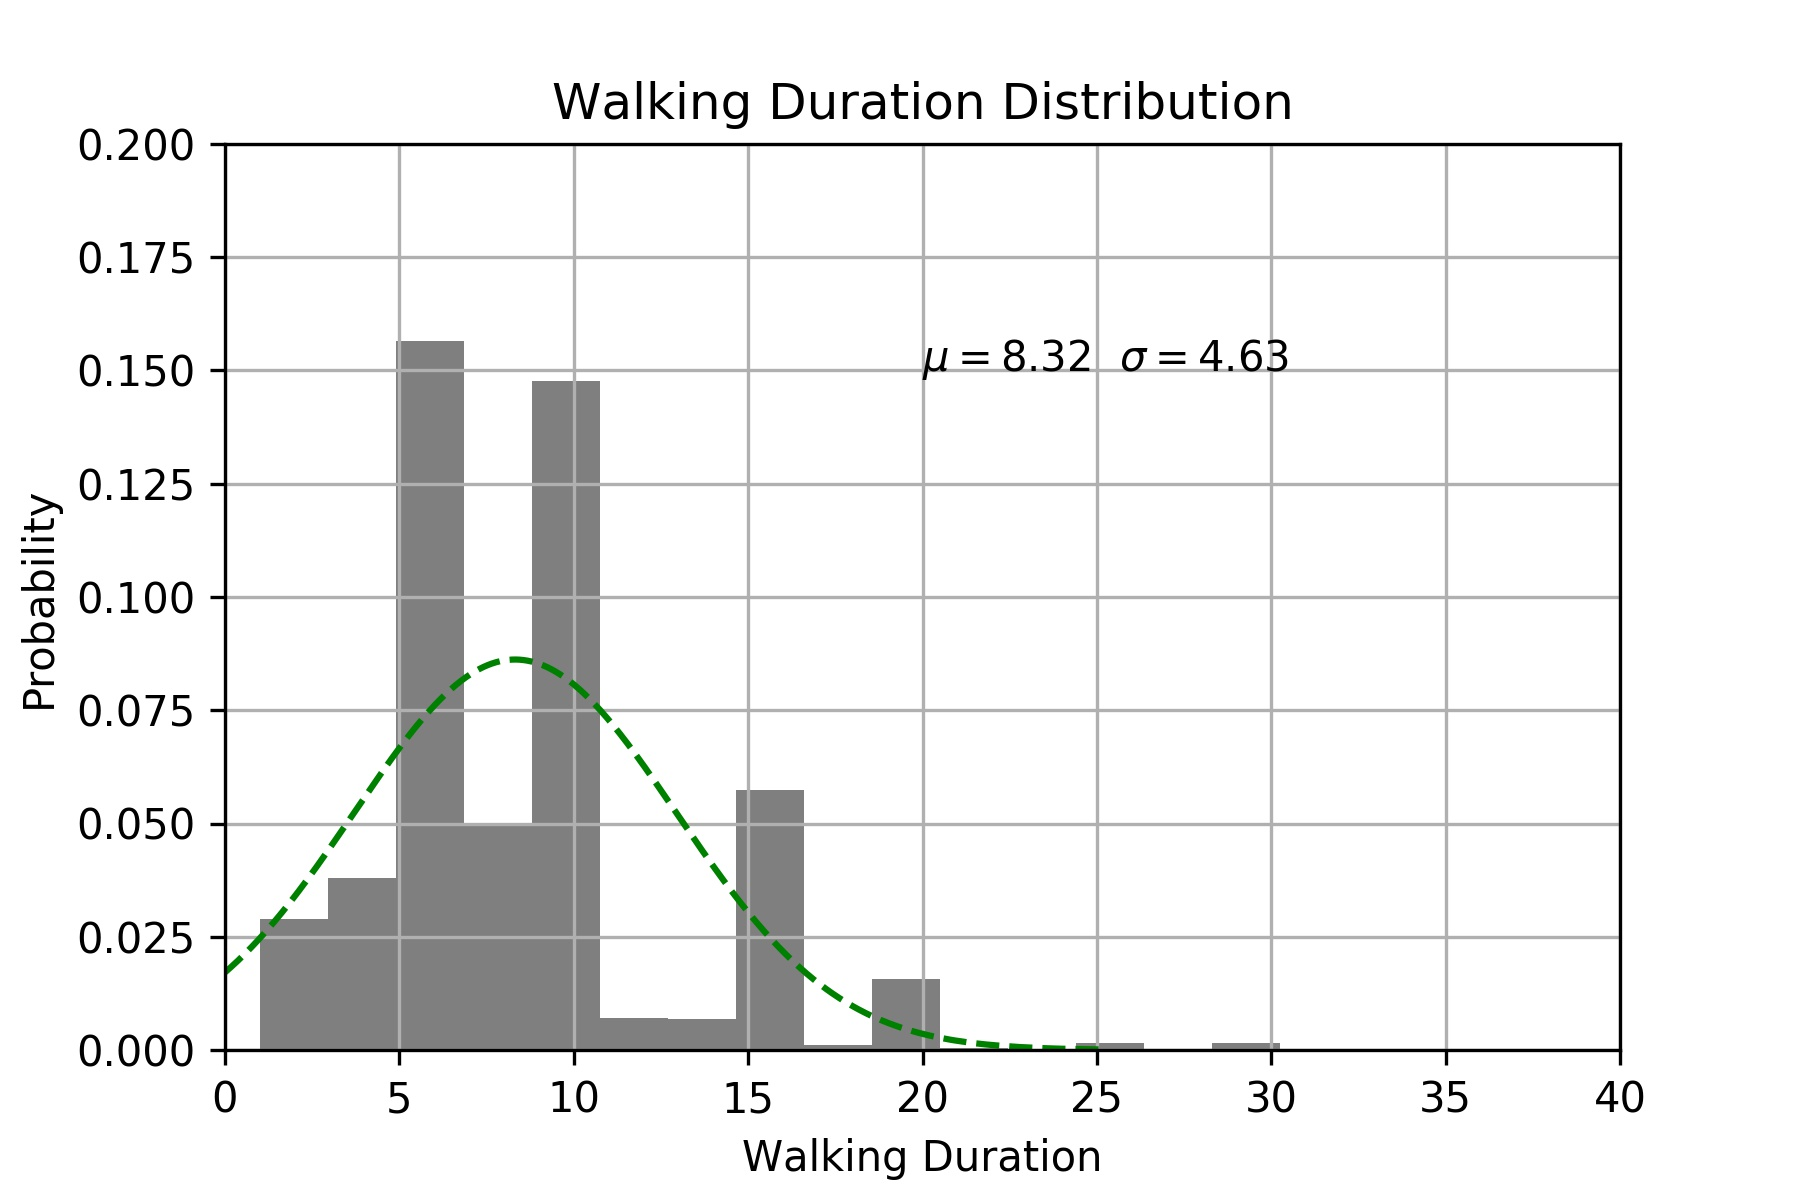
\includegraphics[width=\linewidth]{chp4DurationDistribution}
	\caption{Distribution of Walking Duration}
	\label{fig:chp4:DurationDistribution}
\end{figure}

%
\section{Methods}
%
\subsection{Necessary hypothesis}
Based on the statements outlined in the parts of introduction and review, three basic assumptions are proposed in this study.

\begin{itemize}
	\item A1: The distribution of departures and destinations of people with different individual characteristics in Fukuoka, Japan, is random in space. 
	\item A2: The acceptant walking duration of people with same individual characteristics should subject to the normal distribution. 
	\item A3: The respondents are viewed as they can accept the walking duration that they answered.
\end{itemize}

Based on H1 and H2, when examining the threshold of walking duration $t$, set the proportion of $k$ group in the whole surveyed sample as $r_k$, the proportion of people whose walking durations are under the given threshold of $t$ is marked as $r_{k}^{<t}$, the proportion of people whose walking durations are over the given threshold of $t$ minutes is marked as $r_{k}^{>t}$. If individual characteristics have no significant correlation with acceptant walking durations, there should be no significant differences among $r_k$, $r_{k}^{<t}$, and $r_{k}^{>t}$; otherwise, the three proportion should show significant differences, and the differences will show regularities at different threshold $t$.

Based on H3, if someone gives the answer $t$ minutes, it means this respondent can accept the walking duration of $t$ minutes and any walking duration that less than $t$ minutes. Indeed, this respondent perhaps can accept the walking duration over he answered, but this study just concern about if he can accept the given threshold of the walking duration other than how long he can accept.

%
\subsection{Model}
%
In this study, the variable of walking duration to the rail transit station is a continuous one, while the variables of individual characteristics are multi-categorical, for which the multiple linear regression is considered not applicable. Although there were some studies using the multiple linear regression to estimate the walking duration, the result showed no clear relationship \cite{krygsman2004multimodal}. Since what we concern with is the feature distribution of individual characteristics over or under the thresholds of walking durations, there is no need to find the linear relationship between the individual characteristics and walking durations.

%
According to the assumptions proposed before, when giving a specific threshold of walking duration, passengers walking longer or less than this threshold should have different feature distributions of individual characteristics. That is, if the walking duration of a passenger is more than a given threshold of walking duration, it can be considered that this given threshold of walking duration is an acceptant one, and this passenger should have a relatively high probability of choosing to use rail transit at any threshold of walking duration that less than that given one. This willingness of using rail transit can be reflected by the distribution of walking duration in terms of passengers' individual characteristics, based on which this study examines the relevance of passengers' individual characteristics and this distribution. The abstract model describing this relevance is expressed as follow, of which Equation \ref{eq:chp4:threshold} gives the value of $Y^T_i$, and Equation \ref{eq:chp4:probability} is the probability that $Y^T_i=1$ at given vector of $X_i$.

% & 符号为对齐符号,用于 table 或 matrix
\begin{equation}
    \left\{\begin{matrix}
		Y^T_i=1,&(t_i>T) \\
		Y^T_i=0,&(t_i<T)
	\end{matrix}\right.
	\label{eq:chp4:threshold}
\end{equation}

\begin{equation}
	P(Y^T_i=1 \mid X_i)=F(X_i)
	\label{eq:chp4:probability}
\end{equation}

%
\begin{description}
	\normalsize
	\item[\textbf{Where:}]
	\item[$t_i$] is the walking duration answered by passenger $i$ (in minutes).
	\item[$T$] is the threshold of walking duration that to be examined (in minutes).
	\item[$Y^T_i$] is a binary variable. According to assumption 3, $Y^T_i=1$ means passenger $i$ can accept the threshold of $T$; while $Y^T_i=0$ indicates that it is uncertain whether passenger $i$ can accept this threshold.
	\item[$X_i$] is the vector whose component is the individual characteristics of passengers.
\end{description}

%
The essence of such issue can be viewed as a binary classification problem, for which the models of decision tree, Bayesian, support vector machine (SVM), logistic regression, and neural network are widely adopted. In this study, limited by the volume of sample and features, also the unknown internal relationship among the features, the decision tree model should be a good choice because of the good generalization for different forms of data. Furthermore, to avoid the structure of the tree being too complicated, and to improve the robustness of the model, this study will use an improved model of decision tree, the random forest decision model, to train and test the samples. Random forest decision is an ensemble learning method mainly for classification and prediction. The random forest decision is an extension and improvement for the decision tree model, it is operated by constructing a multitude of decision trees and randomly selecting the features at training time \cite{ho1995random,ho1998random}. To improve the efficiency and accuracy of the model, and reduce the number of invalid branches in the model, it is necessary to filter the invalid features before estimating the model.

%
Briefly, the general process of this study can be summarized as follows. Firstly, data is extracted on the Fukuoka city-wide, including 4254 samples, and 6 main categories of features. Secondly, the features with importance in explaining the willingness of walking duration are selected by using analysis of variance (ANOVA). Thirdly, random forest decision for each threshold of walking duration is estimated, the result obtained from the random forest decision is the probability of walking longer than the given threshold of walking duration for each passenger in terms of individual characteristics. Finally, the accuracy of this result is evaluated using the method of simple moving average by descending order of the predicted probabilities.

%
\section{Results}
The procedure of feature selection includes two parts, the first is the disposal of features with low variance, and the second is the univariate feature selection. The first one is used for filtering the features accounting for very little in the total samples, because a too small quantity in the sample cannot present significant influence on the result. In this study, the multi-categorical features in the original dataset are reclassified into larger groups, thus dealing with the features with low variance. The second step is to select the valid features that indeed have relevance with the independent variable, this step is based on statistical tests. In this study, the Analysis of Variance (ANOVA) is used for estimating the importance of each feature.

%
\subsection{Reclassifying features}
The feature of trip purpose has 15 subcategories in the original dataset, this study reclassifies them into 5 categories including commuting to work, commuting to school, official business, private purpose (such as shopping, entertainment), and going home. The feature of occupation is reclassified from 14 subcategories into 5 categories as well, they are service, technology, administration, student, and the other. Table \ref{tab:chp4:StatisticalDescription} reports some of the statistical description for each feature. Overall, the average walking duration to rail transit stations is 8.32 minutes; more than 75\% of the passengers walk less than 10 minutes; most passengers walk to stations costing 5-10 minutes. In detail, there are some significant differences in the statistical description for each feature, the differences are summarized as follows.

%
\begin{itemize}
	\item People with the purpose of commuting account for the major of rail transit users.
	\item Most people do not accept a more than 15 minutes walking duration to transit stations.
	\item The walking duration in peak hour is longer than off-peak hour.
	\item Young and old people are inclined to spend less time on walking to rail transit stations.
	\item Passengers with the trip purposes of official business and going home tend to take shorter time in walking to rail transit stations.
	\item Passengers with the trip purpose of commuting to work are willing to accept a longer walking duration than that with other purposes significantly.
\end{itemize}


% Table 2
\begin{sidewaystable}[htbp]
	\caption{Statistical Description of Walking Duration for Each Feature}
	\label{tab:chp4:StatisticalDescription}
	\centering
	\small
	\renewcommand{\arraystretch}{1.25}
	\begin{tabular}{llrrccccccc}
		\Xhline{1.5pt}
		Features & Categories & Count & Percentage & Mean & Std & 10th & 25th & 50th & 75th & 90th\\
		
		\midrule
		& Total & 4254 & - & 8.32 & 4.63 & 3 & 5 & 8 & 10 & 15 \\
		
		\midrule
		\multicolumn{1}{l}{Sex}
		& male & 2257 & 53.1\% & 8.41 & 4.63 & 3 & 5 & 8 & 10 & 15 \\
		& female & 1996 & 46.90\% & 8.22  & 4.63 & 3 & 5 & 7 & 10 & 15 \\
		
		\midrule
		\multicolumn{1}{l}{Peak hour}
		& peak & 2976 & 70.00\% & 8.51 & 4.66 & 3 & 5 & 8 & 10 & 15 \\
		& Off peak & 1277 & 30.00\% & 7.88 & 4.52 & 3 & 5 & 7 & 10 & 15 \\
		
		\midrule
		\multicolumn{1}{l}{Age}
		& 5-24 & 543 & 12.80\% & 8.18 & 4.7 & 3 & 5 & 7 & 10 & 15 \\
		& 25-44 & 1992 & 46.80\% & 8.36 & 4.42 & 3 & 5 & 8 & 10 & 15 \\
		& 45-64 & 1407 & 33.10\% & 8.43 & 4.83 & 3 & 5 & 8 & 10 & 15 \\
		& 65- & 311 & 7.30\% & 7.78 & 4.81 & 3 & 5 & 7 & 10 & 15 \\
		
		\midrule
		\multicolumn{1}{l}{Occupation}
		& service & 1256 & 29.50\% & 8.32 & 4.57 & 3 & 5 & 8 & 10 & 15 \\
		& tech & 721 & 17.00\% & 8.58 & 4.89 & 3 & 5 & 8 & 10 & 15 \\
		& office & 1076 & 25.30\% & 8.44 & 4.48 & 4 & 5 & 8 & 10 & 15 \\
		& student & 325 &  7.60\% & 8.12 & 4.73 & 3 & 5 & 7 & 10 & 15 \\
		& null & 875 & 20.60\% & 8.03 & 4.62 & 3 & 5 & 7 & 10 & 15 \\
		
		\midrule
		\multicolumn{1}{l}{Purpose}
		& commuting to work & 2697 & 63.40\% & 8.69 & 4.51 & 4 & 5 & 9 & 10 & 15 \\
		& commuting to school & 287 & 6.70\% & 8.19 & 4.60 & 3 & 5 & 8 & 10 & 15 \\
		& official business & 153 & 3.60\% & 7.10 & 5.05 & 2 & 3 & 5 & 10 & 15 \\
		& private purpose & 789 & 18.60\% & 7.82  & 4.78 & 3 & 5 & 7 & 10 & 15 \\
		& going home & 327 & 7.70\% & 7.17 & 4.67  & 2 & 5 & 5 & 10 & 15 \\
		%
		\Xhline{1.5pt}
	\end{tabular}
\end{sidewaystable}

%
\subsection{Univariate feature selection}
%
According to the achievements from previous studies, the walking distance to rail transit stations ranged generally from 400 meters to 1000 meters in terms of different city types, travel habits, also the needs of research purpose \cite{guerra2012half,murray1998public,o1996walking,keijer2000people,zhao2003forecasting,alshalalfah2007case}. If converting this walking distance into walking duration by using the walking speed of 4.8 km/h, the walking duration would range from 5 minutes to 13 minutes \cite{bohannon1997comfortable}. 

%
In this study, more than 40\% of the samples walk less than 5 minutes, and the walking duration within 13 minutes covers about 85\% of the total. The 5 minutes walking duration can be accepted by most passengers, while a walking duration longer than 13 minutes cannot be accepted by most passengers. In addition, as the average walking duration in this study is about 8 minutes, the three representative thresholds of 5, 8, 13 minutes are picked as the typical threshold for estimating the relationship between individual characteristics and walking durations. 

%
The valid features are identified using ANOVA. The features with p-value less than 0.05, which means this feature relevant with the dependent variable at the confidence level of 95\%, are picked out and listed in Table \ref{tab:chp4:ValidFeatures}. In the Effect column of this table, L means the individual with this feature tend to walk longer than the given threshold of walking duration, while M is the opposite meaning.

% Table 3
\begin{sidewaystable}[htbp]
	\caption{Valid Features and the Effect at Each Threshold}
	\label{tab:chp4:ValidFeatures}
	\centering
	\small
	\renewcommand{\arraystretch}{1.25} % 重设表间距
	
	\begin{tabular}{lrlrlr}
		\Xhline{1.5pt}
		\multicolumn{2}{c}{5 min threshold} & \multicolumn{2}{c}{8 min threshold} & \multicolumn{2}{c}{13 min threshold} \\
		
		\midrule
		Features & Effect* & Features & Effect* & Features & Effect* \\
		Age over 65 & L	& Female & M & Age 45-64 & M \\
		Peak hour & M & Age 25-44 & M & Peak hour & M \\
		O\_Null & L & Peak hour & M & P\_commuting to work & M \\
		P\_commuting to work & M & P\_commuting to work & M & P\_ private purpose & L \\
		P\_official business & L & P\_official business & L	& & \\
		P\_private purpose & L & P\_ private purpose & L & & \\
		P\_going home & L & P\_ going home & L & & \\
		\Xhline{1.5pt}
	\end{tabular}
	%
	\begin{description}
		\normalsize
		\label{note:tab:chp4:ValidFeatures}
		\item[*Note:] L means the individual with this feature tend to walk longer than the given threshold of walking duration, while M is the opposite meaning.
	\end{description}
\end{sidewaystable}

%
As shown in \ref{tab:chp4:ValidFeatures}, at the threshold of 5 minutes, the features of trip purposes and peak hour play the most important role in determining the willingness of walking duration. Situations are changed a little at the threshold of 8 minutes, the importance of age and gender raised in some extent, while the features of trip purposes changed little from that of 5 minutes. The feature importance shows a big difference from 5 and 8 minutes at the threshold of 13 minutes. This result of feature selection is also consistent with common sense and partly confirmed by the previous research. Most of the walking duration is distributed around the average walking duration of 8 minutes, it can be considered that walking duration between 5 and 13 minutes is sensitive to individual characteristics. The walking duration more than 13 minutes is not accepted by most people even if they have different individual characteristics, and the threshold less than 5 minutes is also not sensitive to individual characteristics since the 5 minutes threshold is generally accepted by most passengers.

%
\subsection{Estimation of features}
The valid features (Table \ref{tab:chp4:ValidFeatures}) are used in the random forest decision to estimate the probability that walking longer than the given threshold of walking duration. For estimating the model, the dataset is divided into two parts, 50\% of the sample are used for fitting the model thus obtaining the coefficients, the rest 50\% are used for testing the ability of prediction. The prediction process is presented in Figure \ref{fig:chp4:RandomForests}. For the random forest decision, the prediction is not obtained from the only one decision tree but the multitude of decision trees constructed by random selection of features and samples. The dependent variable at the given threshold of walking duration to rail transit stations is calculated by equation \ref{eq:chp4:probability} based on the mean prediction.

% Figure 5
\begin{figure}[htbp]
	\centering
	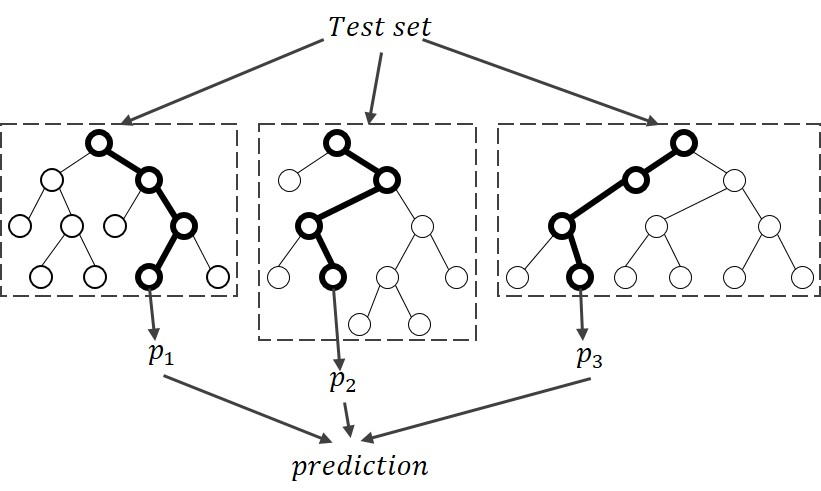
\includegraphics[width=0.7\linewidth]{chp4RandomForests}
	\caption{Prediction Process in Random Forests Decision}
	\label{fig:chp4:RandomForests}
\end{figure}

%
The accuracy of results are evaluated by using the method of simple moving average. Figure \ref{fig:chp4:Prediction} is the trend line of probabilities that walking less than the given threshold. The trend line of the surveyed values based on the test set is calculated by the mean probability of a group people who have close predicted values. The trend line is drawn by a descending order of predicted values. From the comparison of predicted values and surveyed values, it can be known that the prediction at the threshold of 5 minutes has the best fitness, and the prediction for the threshold of 13 minutes is also slightly good, while it is not so good in the case of 8 minutes. In fact, if checking the prediction for individuals, the accuracy of this model is still not enough to explain the individual behavior. But the trend line in Figure \ref{fig:chp4:Prediction} infers that this result can reflect the behavior of people with specific individual characteristics at a given threshold of walking duration. 

% Figure 6
\begin{figure}[htbp]
	\centering
	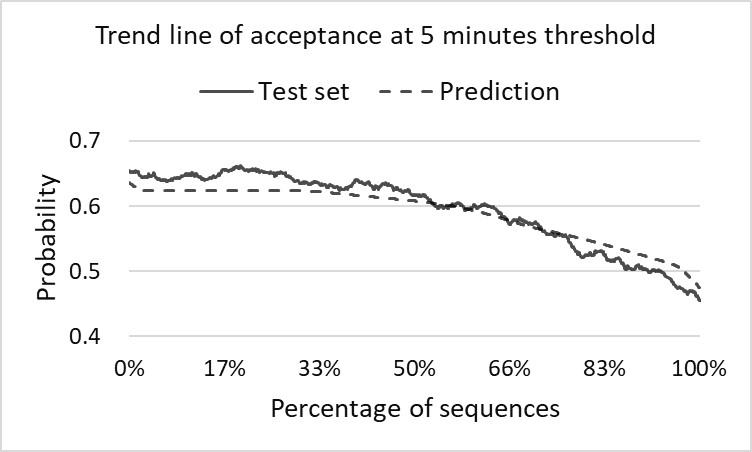
\includegraphics[width=0.7\linewidth]{chp4Prediction5Min} \\
	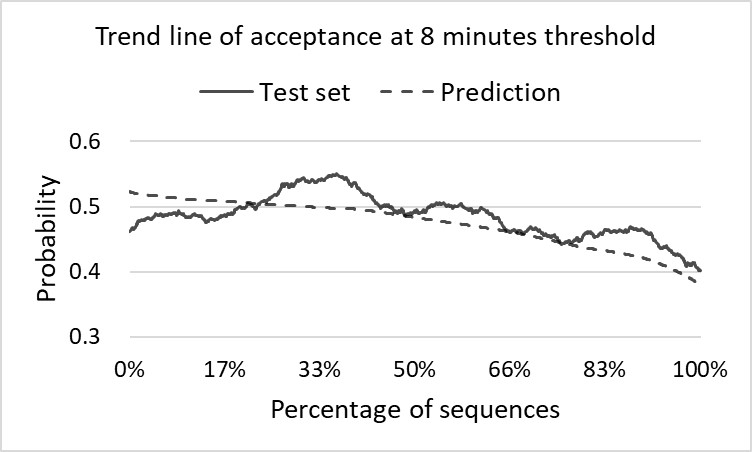
\includegraphics[width=0.7\linewidth]{chp4Prediction8Min} \\
	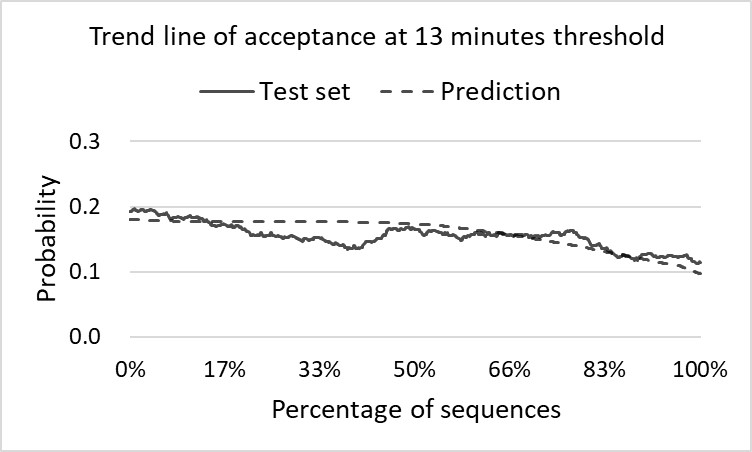
\includegraphics[width=0.7\linewidth]{chp4Prediction13Min} \\
	\caption{Trend Line of Prediction and Test Set}
	\label{fig:chp4:Prediction}
\end{figure}

%
\section{Discussion}
This study described and analyzed 4254 records of rail transit trip. Three thresholds of walking duration are examined. From the result in Table \ref{tab:chp4:ValidFeatures}, trip purpose is the most important factor in determining the walking durations at all the 3 thresholds. The feature of peak hour is also significant in explaining the walking duration. People tend to walk a longer time to stations at peak hours, while people with private purpose or on the way going home are not willing to choose a stations far away. For the details of each threshold, the unemployed people and the elderly people tend to walk less than 5 minutes to stations; people whose age is between 25 and 44 are unwilling to walk more than 8 minutes; people aged from 45 to 64 can accept walking more than 13 minutes to stations more easily.

%
However, summarized above is only the description for the distribution of walking duration in terms of each feature which is hard to apply. In fact, the data in this study is obtained from a factual investigation but not a willingness survey. Once people have made a decision of walking to rail transit stations, the walking duration is just representation of the location of departures and the walking speed. It is hard to say whether the individual characteristics affected the walking durations, maybe due to this reasons few existing studies can explain the relevance between walking duration and individual characteristics quantitatively correctly. The perspective changed a little in this study, under the assumptions proposed before, the distribution of walking duration can be viewed as a reflection of the acceptability of walking duration, which should have relevance with people's individual characteristics. According to assumption 3, the behavior that a passenger chose to walk to a station means this passenger can accept the walking duration from the departure to that station. Based on assumption 1 and 2, if the people who accepted the given threshold of walking duration shows significant differences in individual characteristics, it means they have a different acceptability of walking duration with the others.

%
As explained above, this study examined the differences in individual characteristics of which people who accepted the given thresholds of walking duration. As the results, people with different individual characteristics shows different acceptability at each threshold of walking duration. According to the evaluation from the method of simple moving average, the model of 5 minutes’ threshold has a better explanatory ability, the model of 13 minutes' threshold is a little weaker, and the model of 8 minutes' threshold is not good. Here are some possible reasons for explaining the results. The selected thresholds of walking duration 5, 8, 13 minutes represent the lower boundary, mean value, and upper boundary of the main distribution of walking durations respectively. The commonly acceptable walking durations range from 5 to 13 minutes, therefore, it can be inferred that people who prefer walking less than 5 minutes and who can accept walking longer than 13 minutes may have significant features. However, as the mean value of walking duration, it can be thought that most of the walking durations are distributed around 8 minutes, for passengers there may be some randomness in making the decision of whether walking to rail transit stations. For the other threshold values near the mean value of 8 minutes, it also can be inferred that people may have some ambiguity in choosing whether to walk to stations or not. This explanation can also be confirmed by the result of valid features selection. There are 5 identical features in both thresholds of 5 and 8 minutes, which means people with those features are not sensitive to the threshold from 5 to 8 minutes.

\section{Conclusion}
%
The results of the random forest decision showed good predictive ability for groups of people, especially at the threshold of 5 minutes. However, it did not give ideal results on individual predictions, which means the application of this study needs a certain number of sample scale, there is still a lot of work should be done on improving the accuracy of prediction. In the next stage of this research, we plan to apply the results on predicting the willingness at a specific threshold of walking duration for a group of people. By using this prediction, for example, if knowing the individual characteristics of residents in a particular area locating from the rail transit station $T$ minutes, the general acceptability of walking to the station for the residents in this area should be predictive. Therefore, this prediction of willingness is expected to be used in planning the catchment area of rail transit stations or estimating the catchment area of existing stations.

% reference
\clearpage % 新起一页
\bibliographystyle{apacite}
% \bibliographystyle{IEEEtran}
\bibliography{ref}

\chapter{Influencing Factors on Ridership at Station-to-Station Level}
\markright{CHAPTER 5}

% 待修正,再稍微补充一点,有点短感觉。两段话差不多
\section{Introduction}
% background
\subsection{Background}
%
Urban rail transit is a type of high-capacity public transport generally found in urban areas. Because of the rapid, punctual and environment-friendly features, the urban rail transit is becoming one of the most important travel modes in modern cities. With the popularity of the urban rail transit in modern cities and the emphasis on sustainable development, the concept of TOD (Transit Oriented Development) is put forward, intended to build the compact city \cite{calthorpe1993next}. Many cities around the world have adopted the policy of giving priority to the development of public transport for decreasing the share of motorized travel and increasing the willingness of using public transit. For policymakers, how to grasp the relation between land use and transit ridership has become an important issue that they must face.

%
Although there have been lots of research on the relationship between land use and transit ridership, most of them are conducted from the perspective of the single station. The transit ridership of a station, however, should be affected not only by the elements around that station, but also be affected by the transit ridership of other stations, since all the stations are running in the same system.  Once the circumstance within catchment area changes, obviously, the ridership of this station will change as well. But the increased part of passengers will be transported to other stations, thus every station connected to that station will also have an increase in ridership. 

% why focus on the ridership at station-to-station level
\subsection{Research purpose}
%
Some researchers have discussed on the issue of inter-urban transit demand at station-to-station level \cite{wardman1997inter,jones1983demand}, nevertheless, restricted by the difficulties in collecting data at station-to-station level, few studies focused on intra-urban transit demand \cite{choi2012analysis}. Even now, the transit ridership forecasting at station-to-station level is still difficult due to the complex interaction among stations. 

Based on this realistic background, this study will focus on the relation among stations from the perspective of land use. But rather than making the prediction of transit ridership between station and station, this study tries to explain what factors of land use can influence the choice of destination station for passengers. 

\section{Review}
%
Until now, there are many studies focusing on the relationship between various factors and transit ridership. Most of the studies are based on regression model and conducted from the view of station-level, the transit ridership is thought to be affected by the circumstance surrounding the station \cite{cervero1997travel,taylor2003analyzing,zhao2005transit,estupinan2008relationship,taylor2009nature,sohn2010factors,gutierrez2011transit,jun2015land}. Among them, the multiple linear regression models are the earliest and most widely used model \cite{cervero1997travel,gutierrez2011transit}. However, the data point in ordinary least squares (OLS) model is treated as a single point, which is not consistent with fact since the transit node is connected to each other. To deal with the relationship among stations in the network, the approach of spatial regression is also introduced into this issue \cite{cardozo2012application,jun2015land}. However, this relationship among stations in spatial regression models is just the expression for the distribution relationship of stations in location, it cannot reflect the real connectivity between two station areas.

%
To explore the connectivity between station areas, Choi et al. conducted a station-to-station level investigation into the effect of both origins and destinations on OD metro ridership of Seoul, Korea by using the data from the automatic fare collection system \cite{choi2012analysis}. The factors considered to influence the OD ridership is divided into three groups: the factors of both origin and destination, and the impedance factors between stations. And where the variables of origin and destination are the same, representing the travel characteristics of O and D respectively. The influence of factors on OD ridership is estimated using multiplicative and Poisson regression, with the data of morning, evening peak hours, and midday hours. This station-to-station approach has connected stations by using the factors of both origin and destination. As the result of this empirical study, different land use functions have different travel characteristics in terms of both time and space. However, this approach still cannot reflect the connectivity between two station areas because of the aggregate processing for data.

%
Land use and public transit are coevolving partners in city building \cite{handy2005smart,dittmar2012new}. In the urban railway transit system, the ridership between stations is thought to be related to land use, distribution of functional regions, or travel preferences \cite{thompson1997achieving}. The catchment area of a station is the area with mixed land use of residences, business, and leisure within walking distance taking the station as the center, while the transit ridership between stations can be viewed as the connectivity of different catchment areas. The catchment area is generally referring to a compact residential district that includes mixing land use to allow people to most of their daily activities within the easy walking distance of a major transit node \cite{lund2004travel}. In details, various functional buildings are the carrier for people to live, work and recreate, different functions of buildings correspond different trip purposes. When the functions of buildings within the easy walking distance of a station cannot satisfy the requirement of people’s daily activities, people will choose to go to other places to conduct their business by using the transit node such as the subway. Therefore, the distribution of different functional building in a catchment area is considered to not only affect the ridership of the station where it is located but also affect the ridership of other stations connected to that station.

%
With the goal of explaining the variation in the ridership between stations, this study will focus on the passengers’ choices for destination stations from the perspective of complementarity of building function in different catchment areas, using the case of subway network in Fukuoka, Japan. The result from this study also can provide a foundation for explaining the connectivity between different catchment areas. Factors that are expected to influence the connection of stations are stated in the next section. Then the approach and model that are adopted in this study are interpreted. Based on the approach and model, the case of the subway system in Fukuoka, Japan is investigated. The discussion for the result is also presented in the last section.

%
\section{Data}

%
\subsection{Case introduction}
%
This study focuses on 35 subway stations in Fukuoka City (the sixth largest city in Japan) which has the largest population in Kyushu Island of Japan (more than 1.5 million). Referring to Figure \ref{fig:chp4:ResearchArea}, the research area and the distribution of subway stations. Until now Fukuoka has three operating subway lines, a total of 29.8 kilometers operating mileage. The transport system carries a daily average of more than 0.4 million passengers by 2015 that accounting for more than 20\% in total motorized travel (from Fukuoka City Transportation Bureau). Although the Fukuoka subway system is not a large-scale one, it plays a crucial role in public transportation in terms of the city scale and population. Moreover, one thing should be noted that the third line is not directly connected with the first and second line. The catchment area of transit stations used in this chapter is the same with that in chapter 3. An 800-meter real walking distance on the road network is used as the pedestrian catchment area. The factors considered to have influences on the passengers' choices for destination stations are described as follow.

%
\subsection{Land use factors}
%
Land use is generally accepted as one of the determinants for transit ridership. The indicator of floor area in different building functions can be considered as a detailed expression for land use. Also, many researchers have verified the influence of floor area in different building functions on transit ridership by conducting empirical studies \cite{sohn2010factors,gutierrez2011transit,chakraborty2013land,chakraborty2013land,jun2015land}. Also, all the stations in the network are connected, the change of land use within the PCA of a station will lead to the changes of transit ridership in all the stations in the same network. For the case of Fukuoka, about 90\% of the trips accessing subway stations are non-motorized, in another word, the land use within the PCA of stations play a crucial role in determining the trip purposes of subway users. The accessing duration refers to Table \ref{tab:chp4:AccessToStations}.

%
The same with previous studies, this study chose several types of land use with higher proportion to assess the indicator of land use mix, including residential, office, commercial, education. The four main types of land use account for about 85\% of all the floor area in Fukuoka City, especially in subway PCA, reaching more than 90\%, which refers to Table \ref{tab:chp4:ProportionOfLanduse}. In addition to the indicator of floor area, the index of the land use mix is also assumed to be a crucial factor for explaining the connectivity of stations \cite{badoe2000transportation,cervero2004transit,frank2004obesity}. Different from the general definition of land use mix, this study redefines it into the aggregation of land use. The Euclidean Metric is used for evaluating the deviation of land use aggregation in each subway station with respect to a reference value. The value of this indicator is ranged from 0 to 1, in which the lower value represents a higher diversity in land use function, while the higher value means the land use function is less diverse. This indicator of land use aggregation is defined as for Equation \ref{eq:chp4:LanduseAggregation}, it is speculated to have a negative impact on ridership. To describe the mixture of land use closer to the facts, the referenced balance proportion of land use types is decided by the average proportion of all subway station PCA (800 meters) in Fukuoka City (refer to Table \ref{tab:chp4:ProportionOfLanduse}). There are five variables of land use category selected as the indicator in this study, the list of indicators also the statistical descriptions refer Table \ref{tab:chp5:StationToStationFactorStatistics}.

% Table
\begin{table}[htbp]
	\centering
	\caption{Statistical description of data}
	\label{tab:chp5:StationToStationFactorStatistics}%
	\small
	\renewcommand{\arraystretch}{1.25} % 重设表间距
	\begin{tabular}{llrp{5em}<{\raggedleft}p{5em}<{\raggedleft}p{5em}<{\raggedleft}} 
		\Xhline{1.5pt}
		Category & Variable & Unit & Min Value & Max Value & Average \\
		
		\midrule
		\multirow{4}[0]{*}{Land use}
		& Commerce & \% & 1.03 & 44.58 & 9.89 \\
		& Office & \% & 0.41 & 44.19 & 12.78 \\
		& Residence & \% & 7.15 & 92.26 & 60.34 \\
		& Education & \% & 0.03 & 48.02 & 7.08 \\
		& Land Use Aggregation & - & 0.09 & 0.75 & 0.31 \\
		
		\Xhline{0.5pt}	
		\multirow{2}[0]{*}{Impedance} 
		& Bus Capacity & - & 58.48 & 2.91 & 259.80 \\
		& Bus Accessibility & - & 89.71 & 4.00 & 455.00 \\
		& Operation Distance & $km$ & 154.50 & 389.30 & 237.58 \\
		\Xhline{1.5pt}
		
	\end{tabular}%
\end{table}%

%
\subsection{Impedance factors}
%
Another factor generally used for representing the connectivity between stations is the remoteness, which is also widely adopted as impedance in the gravity model for explaining the connectivity between traffic zones \cite{iwanow2007trade,kepaptsoglou2010gravity,nitsch2000national}. Impedance is the index that represents the connectivity and cost between origin and destination, it can affect the choice of the trip in terms of both destination and travel mode. Generally, the factor of impedance can be considered from two aspects in this issue, one is the internal impedance that representing the convenience for accessing the station \cite{chu2004ridership,chakraborty2013land}; the other is external impedance that evaluating the connectivity between stations \cite{sohn2010factors}.

%
For Fukuoka, there are about 90\% of all the trip accessing stations by walking and bicycles (refer to Table \ref{tab:chp4:AccessToStations}). Because the PCA is set by the pedestrian distance, the internal road impedance has been already considered in the phase of setting the PCA. It can be thought that there is no need to create a new indicator to represent the internal impedance in this case study.

%
Since the focus of this study is the connectivity between stations, it can be assumed that the interconnection between stations in a subway network is an influential factor in determining the ridership between stations. Two types of external impedance are considered in this study. The operation distance of subway line between two stations is the direct indicator representing the spatial connectivity between two stations. And the impedance of competing modes is also considered in this study. Two indicators of bus accessibility and bus capacity are proposed referring to Equation \ref{eq:chp4:BusCapacity} and Equation \ref{eq:chp4:BusAccessibility} respectively. The former one is used for representing the convenience for accessing the station which is speculated as a positive factor for ridership, while the later one is the transport capacity of the bus within the PCA of the station which is considered as a negative factor for ridership because it may share part of ridership from the subway. All the statistical description of indicators in this study are listed in Table \ref{tab:chp5:StationToStationFactorStatistics}.

%
\section{Methods}
%
\subsection{Flow of the method}
It is difficult to analyze the connectivity of all the stations simultaneously. To simplify this issue, the study will be started by one single station, and then the connectivity between this station and all the other stations connected to it will be investigated. For a passenger, the behavior of going to some places by subway can be viewed as a procedure of choice. In this selection process, the choice is decided by the trip purpose of the passenger. As stated in the introduction, the type of building functions can be mainly categorized into residence, office, education, and commerce, which represent the trip purposes of going home, business, commute, and leisure respectively. Therefore, this issue can be converted into a discrete choice model, in which the dependent variables are the building environment in the station catchment area, and the independent variable is the choice of the destination station.

%
\subsection{Logistic regression}
Taking one station as the destination station, it will correspond to the other departure stations in the subway system. The passengers from the all the departure stations have two options at that destination station, that is getting off and not getting off at this destination station. This probability of getting off at that destination station can be viewed as the representation of the connectivity between the departure station and the destination station. At this point, this issue has been converted into a binary choice problem that investigating the probability of getting off at one subway station. Thus, the Binary-Logistic Regression is introduced into this study to deal with this issue. Formula \ref{eq:chp5:LogisticRegression} shows the Binary-Logistic Regression that will be adopted in the next section.

% Equation 4
\begin{equation}
	p_i(y_i=1 \mid X_i)=\frac{1}{1+e^{-(\alpha +X_i)}}
	\label{eq:chp5:LogisticRegression}
\end{equation}

\begin{description}
	\setlength{\parskip}{0\baselineskip} % 设置段间距
	\normalsize
	\item[\textbf{Where:}]
	\item[$p_i$] is the probability of getting off the subway for the $i$th passenger.
	\item[$y$] is the choice of passengers.
	\item[$X_i$] is the attribute vector of the $i$th passenger.
	\item[$\alpha$] is the residual item
	\setlength{\parskip}{0.7\baselineskip} % 设置段间距
\end{description}

%
For the estimation of a regression model, the model of logistic regression built in this study is a non-linear regression model, which can be directly estimated by using maximum likelihood estimation (MLE). Thus, the MLE is adopted to estimate the coefficient. In this study, the sample size is the passenger volume of all the departure stations connected to the investigated destination station, which is marked as $N$. The same with Equation \ref{eq:chp5:LogisticRegression}, $p_i$ is the probability for choosing to get off, thus, $1-p_i$ represent the probability for choosing not to get off. Then the occurrence probability $L(\theta)$ in all observation sample can be expressed as Equation \ref{eq:chp5:MLE}:

% Equation 5
\begin{equation}
	L(\theta)=\prod_{i=1}^{N}{p_i}^{y_i}(1-p_i)^{(1-y_i)}
	\label{eq:chp5:MLE}
\end{equation}

\begin{description}
	\setlength{\parskip}{0\baselineskip} % 设置段间距
	\normalsize
	\item[\textbf{Where:}]
	\item[$p_i$] is the probability of getting off at the investigated destination station for the $i$th passenger.
	\item[$y_i$] is the choice of $i$th passenger, of which $y_i = 1$ means getting off at the investigated destination station, $y_i = 0$ means not getting off at the investigated station.
	\item[$N$] is the number of passengers riding rail transit at all the departure stations connected to the investigated destination station
	\setlength{\parskip}{0.7\baselineskip} % 设置段间距
\end{description}

\section{Results}
%
The characteristic of land use within the PCA of a station can represent the characteristic of passengers departing from that station. Since a city is the collection of different functional regions, the land use characteristics of each PCA are also different. To explore the connectivity between stations with different types of land use characteristics, this study firstly classifies all the stations in terms of the proportion of different function of land use and population density. Then the typical stations are chosen from each group of different land use type, thereby estimating the connectivity between stations by conducting the logistic regression. 

\subsection{Selection of object station}
%
As the result, all the stations are fallen into six categories, they are medium-density residence, high-density residence, education, office, commerce, and airport (refer to Figure \ref{fig:chp3:StationClassification}). Detailed statistics for each type is shown in Table \ref{tab:chp5:StationClassification}, the average values of attributions in each group are represented, furthermore, the factors of bus service and land use aggregation are also put in this table to help to observe the difference among groups. As is shown, both the group of medium-density residence and the group of high-density residence have a higher proportion of residence floor area, but there is a significant difference in the population density in the two groups. It is clearly that the education type has the highest proportion of education floor area. Both the office type and the commerce type have a higher proportion in office than other types, but the commerce proportion in commerce type is also higher than other types. Additionally, the station of Fukuoka airport does not belong to any group, which mainly takes the feeder traffic from the airport to urban area. It also can be noted that the residence and office type have a relatively lower land use aggregation and higher population density.

% Table 3
\begin{sidewaystable}[htbp]
	\centering
	\caption{Station classification}
	\label{tab:chp5:StationClassification}
	\small
	\renewcommand{\arraystretch}{1.25} % 重设表间距
	\begin{tabular}{p{12em}<{\raggedright}p{4em}<{\centering}p{4em}<{\centering}p{4em}<{\centering}p{4em}<{\centering}p{4em}<{\centering}p{5em}<{\centering}p{5em}<{\centering}p{5em}<{\centering}}
		
		\Xhline{1.5pt}
		Type & Population density & Commerce & Office & Residence & Education & Land Use Aggregation & Bus Capacity & Bus Accessibility \\
		\midrule
		
		Medium-density residence & 98 & 4\% & 3\% & \cellcolor[rgb]{.8, .8, .8} 83\% & 4\% & 0.34 & 18 & 28 \\
		High-density residence & 173 & 5\% & 7\% & \cellcolor[rgb]{.8, .8, .8} 76\% & 6\% & 0.26 & 51 & 80 \\
		Education & 83 & 5\% & 6\% & 51\% & \cellcolor[rgb]{.8, .8, .8} 22\% & 0.3 & 45 & 52 \\
		Office & 135 & 8\% & \cellcolor[rgb]{.8, .8, .8} 31\% & 49\% & 3\% & 0.18 & 83 & 131 \\
		Commerce & 69 & \cellcolor[rgb]{.8, .8, .8} 34\% & \cellcolor[rgb]{.8, .8, .8} 32\% & 24\% & 1\% & 0.47 & 132 & 213 \\
		Airport & 36 & 1\% & 3\% & 45\% & 2\% & 0.23 & 32 & 56 \\
		\Xhline{1.5pt}
		
	\end{tabular}
	%
	\begin{description}
		\small
		\label{note:tab:chp5:StationClassification}
		\item[Note:] the highlighted cells refer to the representative values that having much higher percentage than other land use types.
	\end{description}
	
\end{sidewaystable}

%
To investigate the stations with significant differences in land use characteristic, the most typical object station is chosen from each group in terms of the guidelines as follow. 1) Avoid selecting the stations with the highest value of feature indicator. Because the high value may be caused by the particularity of its distribution of land use and road network, it does not have generality in terms of the type it is. 2) Avoid selecting the transferable stations. Because the transit ridership of this kind of stations generally relates the other stations, which cannot reflect the distribution of land use within the PCA. 3) Avoid selecting the stations with much lower or higher population density than other stations. Because the low or high population density may lead to different travel preference due to the difference in the distribution of facilities (such as hospitals, schools, and transportation facilities etc.). Finally, six stations are selected from six groups, the factor of each station is shown in Table \ref{tab:chp5:Result}.

% Table 4
\begin{sidewaystable}[htbp]
	\centering
	\caption{Result of Logistic Regression}
	\label{tab:chp5:Result}
	\footnotesize % 该表使用小字体
	\renewcommand{\arraystretch}{1.25} % 重设表间距
	
	\begin{tabular}{p{7em}p{5em}p{5em}<{\centering}rrrrrrrrr}
		\Xhline{1.5pt}
		
		% 表题第一行
		\multicolumn{2}{c}{Destination Station} & & \multicolumn{9}{c}{Variables in Boarding Station} \\
		\midrule
		
		% 表题第二行
		\multirow{2}[5]{7em}{Type} & \multirow{2}[5]{5em}{Station} & \multirow{2}[5]{5em}{\centering{Statistical index}} & \multicolumn{5}{c}{Land use} & & \multicolumn{3}{c}{Impedance} \\
		\cmidrule{4-8} \cmidrule{10-12}
		
		% 表题第三行
		& & & 
		\multicolumn{1}{p{5em}}{\centering{Commerce}} & 
		\multicolumn{1}{p{5em}}{\centering{Office}} & 
		\multicolumn{1}{p{5em}}{\centering{Residence}} & 
		\multicolumn{1}{p{5em}}{\centering{Education}} & 
		\multicolumn{1}{p{5em}}{\centering{Land use Aggregation}} & &  \multicolumn{1}{p{5em}}{\centering{Distance}} & 
		\multicolumn{1}{p{5em}}{\centering{Bus Capacity}} & 
		\multicolumn{1}{p{5em}}{\centering{Bus Accessibility}} \\
		\midrule
		
		% 开始表的内容
		\multirow{3}[0]{7em}{Medium-density residence} & \multirow{3}[0]{5em}{Kamo} & \textsl{B} & -0.05 & -0.06 & -0.06 & -0.07 & -0.03 & & 0.07 & 0.01 & -0.01 \\
		& & \textsl{P-value} & 0.00 & 0.00 & 0.00 & 0.00 & 0.00 & & 0.00 & 0.04 & 0.04 \\
		& & \textsl{Exp(B)} & 0.95 & 0.94 & 0.94 & 0.93 & 0.97 & & 1.07 & 1.01 & 1.00 \\
		\midrule
		
		\multirow{3}[0]{7em}{High-density residence} & \multirow{3}[0]{5em}{Fujisaki} & \textsl{B} & 0.01 & \cellcolor[rgb]{.8, .8, .8} 0.00 & -0.01 & 0.01 & -0.02 & & -0.06 & 0.00 & 0.00 \\
		& & \textsl{P-value} & 0.00 & \cellcolor[rgb]{.8, .8, .8} 0.18 & 0.00 & 0.00 & 0.00 & & 0.00 & 0.00 & 0.00 \\
		& & \textsl{Exp(B)} & 1.01 & \cellcolor[rgb]{.8, .8, .8} 1.00 & 0.99 & 1.01 & 0.98 & & 0.95 & 1.00 & 1.00 \\
		\midrule
		
		\multirow{3}[0]{7em}{Education} & \multirow{3}[0]{5em}{Hakozakikyudai} & \textsl{B} & 0.02 & \cellcolor[rgb]{.8, .8, .8} 0.00 & 0.02 & 0.03 & -0.01 & & -0.13 & 0.00 & 0.00 \\
		& & \textsl{P-value} & 0.00 & \cellcolor[rgb]{.8, .8, .8} 0.53 & 0.00 & 0.00 & 0.00 & & 0.00 & 0.04 & 0.00 \\
		& & \textsl{Exp(B)} & 1.02 & \cellcolor[rgb]{.8, .8, .8} 1.00 & 1.02 & 1.03 & 0.99 & & 0.88 & 1.00 & 1.00 \\
		\midrule
		
		\multirow{3}[0]{7em}{Office} & \multirow{3}[0]{5em}{Gofukumachi} & \textsl{B} & 0.02 & -0.02 & 0.02 & 0.05 & -0.01 & & \cellcolor[rgb]{.8, .8, .8} -0.01 & 0.00 & 0.00 \\
		& & \textsl{P-value} & 0.00 & 0.00 & 0.00 & 0.00 & 0.01 & & \cellcolor[rgb]{.8, .8, .8} 0.72 & 0.03 & 0.00 \\
		& & \textsl{Exp(B)} & 1.02 & 0.98 & 1.02 & 1.06 & 0.99 & & \cellcolor[rgb]{.8, .8, .8} 0.99 & 1.00 & 1.00 \\
		\midrule
		
		\multirow{3}[0]{7em}{Commerce} & \multirow{3}[0]{5em}{Tenjinn} & \textsl{B} & -0.01 & -0.01 & 0.01  & 0.03  & 0.02  & & 0.06 & \cellcolor[rgb]{.8, .8, .8} 0.00 & 0.00 \\
		& & \textsl{P-value} & 0.00 & 0.00 & 0.00 & 0.00  & 0.00 & & 0.00 & \cellcolor[rgb]{.8, .8, .8} 0.38 & 0.00 \\
		& & \textsl{Exp(B)} & 1 & 0.99 & 1.01 & 1.03 & 1.02 & & 1.06 & \cellcolor[rgb]{.8, .8, .8} 1.00 & 1.00 \\
		\midrule
		
		\multirow{3}[0]{7em}{Airport} & \multirow{3}[0]{5em}{Fukuoka Airport} & \textsl{B} & -0.03 & 0.03 & -0.01 & -0.02 & 0.03 & & -0.08 & 0.00 & 0.00 \\
		& & \textsl{P-value} & 0.00 & 0.00 & 0.00 & 0.00 & 0.00 & & 0.00 & 0.00 & 0.00 \\
		& & \textsl{Exp(B)} & 0.97 & 1.03 & 0.99 & 0.99 & 1.03 & & 0.92 & 1.00 & 1.00 \\
		\Xhline{1.5pt}
		
	\end{tabular}%
%
	\begin{description}
		\footnotesize
		\label{note:tab:chp5:Result}
		\item[Note:]
		$B$ is the coefficient \\
		$Exp(B)$ is the odds ratio \\
		Gray cell means the estimated value is not significant at the significance level of 0.05 \\
	\end{description}
	
\end{sidewaystable}%

\subsection{Estimation of logistic regression}
%
In this study, the independent variable is the choice of getting off at the object station or not, and the influencing factors are land use and impedance between stations and stations. Notably, in the case of Fukuoka subway network, subway line 3 is not directly connected with that line 1 and line 2, thus subway line 3 is addressed separately from subway line 1 and line 2. That is, if the object station belongs to subway line 3, the connectivity will be only investigated within subway line 3. The result of estimation is shown in Table \ref{tab:chp5:Result}.

%
The estimation is as shown in Table \ref{tab:chp5:Result}, the values in gray cell mean that this factor showed no statistical significance at the confidence level of 0.05. The index of $Exp(B)$, which is the odds ratio, represents the extent to the effect on the probability of choice if the coefficient $B$ changes one unit. Here giving a brief explanation of the index of $Exp(B)$, since the unit and meaning of the variables entered the models are different. For the variables of land use, the index of $Exp(B)$ represents that the 1 percent (0.01 unit) change in the variables will lead to an $Exp(B)$ multiples of increases in the probability of getting off at the object station. For the variables of impedance, it means the 1 unit change in the variables will lead to an $Exp(B)$ multiples of increases in the probability of choosing the object station as a destination. 

%
A further explanation taking the Tenjin station as an example is given as below. From the point of land use, the increase of commerce and office floor area in the catchment area of the boarding stations can lead to a decrease in the probability of choosing the Tenjin station as the destination station; while the increase of residence and education floor area in the catchment area of boarding stations can raise the probability of choosing to go the Tenjin station. If interpreted in terms of connectivity, the business type of Tenjin Station is weakly connected to stations with the same commercial type, and the stations of office type; while the stations of business type have relatively strong connectivity with the stations of residence and education type. 

%
\section{Discussion}
%
From the perspective of TOD, this study investigated the connectivity between stations with different land use characteristic by examining the impact of land use and impedance on subway passengers' choice of the destination station. As shown in Table \ref{tab:chp5:StationClassification}, the PCA of the station in Fukuoka shows a significant characteristic of land use distribution, and all the subway stations are categorized into six major types. The result of logistic regression shows the coefficient of factor influencing the choice of the destination station, which can be explained as the connectivity between different PCAs.

%
Some findings of the land use factors can be known from the result in Table \ref{tab:chp5:Result}. The increase in the proportion of residence area of the departure station can lead to an increase in the choice of taking the office and education type station as destination stations. This can be explained as the result of commuter traffic since there is a relatively stronger connectivity between the residential area and work area \cite{badoe2000transportation}. But the situation may change in the medium-residence type due to the different travel preferences in the area with different population density. Another interesting finding is that all kinds of land use have positive connectivity with the education type station. One speculation is that students tend to take public transit because of the low income. Overall, one kind of land use generally shows a rejection effect on the station which has a similar consist of land use type. Such as the Tenjin station located in the CBD area, the proportion of commerce area in the PCA of departure station causes a negative effect on the choice of getting off at Tenjin station. Moreover, the variable of land use aggregation shows that there is a positive connectivity between the areas with an unbalanced distribution of land use.

%
The factors of impedance also showed a good statistical significance, however, the results do not seem to show a certain regularity in different types of stations. Here some possible speculations of the reasons are given for helping to find the limitation of this study and explore the direction for the next study. First, the share of different transportation modes is not considered in this study. The distance between two stations may also affect the variation in the share of different transportation modes, thus it is not stable in representing the impedance.  Second, the variables of bus service describe the features of one single station, but not the features that reflecting the connectivity between two stations. If considering two stations, one is in the downtown where the transportation hub locates, and one is in suburban where there are few public transportation facilities; it can be inferred that even though the bus service is rich in the downtown area, it affects very little on the station located in the suburban area.

%
\section{Conclusion}
%
This study investigated the effect of land use and impedance between stations on the OD subway ridership from the perspective of the connectivity. The effect of factors on the choice of destination station was estimated using the logistic regression model. The result showed that the influence of land use on the ridership between stations was effective, and this result could be explained consistently with fact; while the factor of impedance was still difficult to get explained.

%
From the results obtained in this article, in the urban rail transit, the land use within the station catchment area is an important factor in determining the destination of passengers. Correspondingly, the change in the choice of destination can be reflected to the transit ridership. Furthermore, this change in the transit ridership of each station, which is caused by the change in the choice of destination, is the reflect of the connectivity between the station and the station in terms of land use in each station catchment area. The results are clearly shown in Table \ref{tab:chp5:Result}.

%
Based on the results in this study, the next stage of this research will focus on the share ratio in different transportation modes to make a deeper exploration of subway ridership. The factor of impedance will also be rebuilt to help to describe the connectivity between stations more accurately.

% reference
\clearpage % 新起一页
\bibliographystyle{apacite}
% \bibliographystyle{IEEEtran}
\bibliography{ref}

% 参考文献放在frontmatter部分会出现如下的页码问题。总参考文献如果放入backmatter部分就没问题了。不过这部分注释作为插入页码的方法保留一下。
% \clearpage % 需要另起一页,不然页码会出错
% \addcontentsline{toc}{chapter}{References} % 将reference加入目录。这里addcontentsline之后马上加入目录。
% \bibliographystyle{apacite}
% \bibliography{ref}

% 标记为后记部分
\backmatter
% \setlength{\parskip}{0\baselineskip} % 设置段间距还原为0
% \bibliographystyle{apacite}
% \bibliography{ref}
% \appendix
% \chapter{Appendix}

\end{document}

% 以下是自己做的一个表页,暂时弃用
% Not the standard layout
%\thispagestyle{empty}
%\vspace{\fill}
%{
%	% Format
%	\centering
%	\Large
%	
%	% Title
%	{\huge Dissertation title: may be long or short}
%	\vspace{2cm}
%	
%	
\includegraphics[scale=0.2]{university.jpg}
%	\vspace{2cm}
%	
%	% Author
%	{\LARGE Chen Qi}
%	\vspace{2cm}
%	
%	% Institution
%	Graduate School of Human-Environment Studies\\
%	Kyushu University\\
%	\vspace{2cm}
%	
%	% Supervisor
%	Supervisor: Prof. Zhao Shichen\\
%}
%
%\vspace{\fill}
%\centering\today
